\PassOptionsToPackage{table}{xcolor}
\documentclass[11pt,a4paper]{article}

\usepackage[margin=2.5cm]{geometry}
\usepackage{todonotes}
\usepackage{microtype}
\usepackage{amssymb,amsmath}
\usepackage{pifont}
\usepackage{mathpazo}
\usepackage{accents}
\usepackage{longtable,booktabs}
\usepackage{pgf}
\usetikzlibrary{shapes.geometric}
\usetikzlibrary{matrix}
\usepackage{pgfplots}
\pgfplotsset{compat=1.18}
\usepackage{natbib}
\usepackage{hyperref}
\usepackage[capitalise,noabbrev,nameinlink]{cleveref}
\usepackage{parskip}
\usepackage{xcolor}
\usepackage{changelog}
\usepackage{tcolorbox}
\usepackage{caption}
\usepackage{float}
\hypersetup{
  pdftitle={Storing the Cardano ledger state on disk: requirements for high performance backend},
  pdfborder={0 0 0},
  breaklinks=true
}

\newcommand\deltavar[1]{\accentset{\Delta}{#1}}

\begin{document}

\title{Storing the Cardano ledger state on disk: \\
       requirements for high performance backend}
\date{Version 1.0, April 2025}
\author{Duncan Coutts \\ {\small \texttt{duncan@well-typed.com}} \\
                         {\small \texttt{duncan.coutts@iohk.io}}
       }

\maketitle

\begin{changelog}[simple, sectioncmd=\section*]
  \shortversion{author=Joris Dral, v=1.0, date=April 2025, changes=Editorial changes}
  \shortversion{author=Duncan Coutts, v=0.9, date=July 2023, changes=Final version}
\end{changelog}

\setcounter{tocdepth}{2}
\tableofcontents

\section{Executive summary}

The project to reduce the Cardano node's memory use (known informally as
``UTxO HD''\footnote{Connoisseurs of bad jargon may be interested to note that
this term is a double misnomer. UTxO HD refers to moving the UTxO to the hard
disk, however the the UTxO is only half of the ledger state that the project
aims to deal with, and the UTxO cannot be stored on a hard disk because
spinning hard disks are far too slow to meet the minimum performance
requirements.}) has taken the approach of building an interim solution (MVP) as
a major step towards the complete solution.

The interim (MVP) solution:
\begin{enumerate}
\item is largely complete (at the time of writing);
\item moves approximately half of the ledger state to disk (the UTxO itself);
      and
\item uses an adequate low performance on-disk storage backend (based on LMDB)
      without support for comprehensive I/O fault testing.
\end{enumerate}

The MVP is suitable for deployment as an interim solution:
\begin{itemize}
\item It reduces the node's memory use by approximately 40\%, from 13Gb to 8Gb.
\item It increases the node's blockchain synchronisation time by approximately
      25\%, from approximately 21 to 26 hours. Some regression in
      synchronisation time was expected. A regression of 25\% is not ideal but
      has been deemed acceptable.
\end{itemize}
The MVP will not remain suitable indefinitely however.
\begin{itemize}
\item The node's performance and memory use will degrade as the UTxO scales
      with more users.
\item The MVP cannot \emph{simultaneously} meet all of the performance targets
      from the business requirements, even at the minimum `threshold' level.
\end{itemize}
Fundamentally, Cardano \emph{cannot scale} to its intended number of users
(e.g. Bitcoin or Ethereum size) without completing the project to satisfy the
various business requirements.

It is recommended that the project continue to the complete solution, which
will involve:
\begin{enumerate}
\item moving the remaining large parts of the ledger state to disk; and
\item implementing and integrating a high performance on-disk storage backend
      with support for comprehensive I/O fault testing.
\end{enumerate}
These two parts of the project are both substantial: they are likely to take
several months each with a small team. They can run concurrently or
sequentially, with some efficiency savings if done sequentially but taking
longer overall. The implementation of the high performance on-disk storage
backend can be done as an `arms length' activity and thus could be outsourced.
All other parts will at require significant work from the existing ledger and
consensus teams, though with the possibility of extra help.

The focus of this document is on the improved on-disk storage backend, but
the other half of the project should be kept in mind. The improved on-disk
storage backend is intended to have two main benefits:
\begin{enumerate}
\item it should enable the node to meet its performance and scaling targets,
      which will allow Cardano to scale to many more users while remaining
      within reasonable memory limits;
\item it should restore the comprehensive I/O fault testing for the consensus
      layer which would assure the continued robustness of the node to I/O
      errors and silent disk corruption.
\end{enumerate}

\section{Risks to the status quo}

There are a number of risks if the MVP remains as the status quo
\begin{itemize}
\item As the number of users and wallets increases, the node's memory use (RAM)
      will also increase because the large stake related tables are still kept
      in memory.

      The solution is to move the remaining stake tables to disk.
      See \cref{sec:single-table-design-shortcut} for details.

\item The time taken for the node to synchronise will degrade as the size of
      the UTxO grows beyond what can fit in memory (i.e. with more use and more
      users). It can be expected to degrade to the point where the node does
      not meet its threshold (i.e. minimum) business requirement targets for
      the combination of memory use, UTxO size and synchronisation performance.

      The solution is to implement and integrate a higher performance on-disk
      backend. See \cref{sec:lmdb-backend-shortcut}
      and \cref{sec:performance-limits-of-the-lmdb-backend} for details.

\item A compromise in the MVP is that the node can no longer be comprehensively
      tested for being robust against disk I/O errors and disk corruption. Over
      time, without the ability to test, this is likely to lead to a lack of
      robustness and hence more frequent problems for node users, user
      dissatisfaction and increased support load.

      The solution is to implement and integrate a new on-disk backend that can
      use the existing I/O fault testing framework, restoring the ability of
      the consensus layer as a whole to be tested. See \cref{sec:assurance}
      for details.

\item There is an existing security risk to do with switching between chain
      forks sufficiently quickly to meet Ouroboros Praos security assumptions.
      It is not always possible to switch between different chain forks as
      quickly as the Ouroboros Praos security analysis assumes. The risk
      arising as a consequence of failing to meet this assumption is
      unfortunately difficult to quantify. It is clear however that a
      regression in synchronisation speed corresponds to switching forks more
      slowly, which increases the risk. The MVP has a 25\% regression in
      synchronisation speed and thus a similar regression is expected in the
      time to switch forks. As noted above this is expected to get worse as the
      UTxO continues to grow. The consequences and severity of this risk are
      still being analysed by the Ouroboros researchers.

      Though the risk is hard to quantify, it is clear that the risk can be
      mitigated by improving the synchronisation speed. Part of that involves
      integrating a new on-disk backend that will not regress further as the
      UTxO grows. Another part would be to improve synchronisation speed by
      taking advantage of CPU and I/O parallelism. See
      \cref{sec:blockchain-fork-switching,sec:a-possible-approach-to-io-pipelining-in-the-consensus-layer}
      for details.

\end{itemize}

\section{Summary of benefits}

The improved on-disk storage backend is intended to have three main benefits.
\begin{enumerate}
\item It should achieve substantially higher throughput for crucial operations,
      while also using less memory and scaling to much bigger on-disk tables.

      This would have the following benefits.
      \begin{itemize}
      \item It should enable Cardano to scale to a much larger UTxO size --
            comparable with that of Bitcoin -- and thus scale to many more
            users.
      \item It should stop the current trend of node operators having to use
            ever more capable and expense hardware or VMs with more and more
            memory as the size of the UTxO grows. Indeed it should allow
            operations to use cheaper VMs compared to what is currently the case.
      \item It should enable the current node's consensus layer to achieve
            faster blockchain synchronisation times than with the existing
            low-performance backend.
      \item It should achieve faster chain replay and revalidation times.
      \item It should enable the node to meet its `middle' performance targets
            with the minimum required hardware and the `stretch' targets with
            higher performance SSD hardware.
      \item It should avoid the additional regression in synchronisation (and
            replay and revalidation) times that is anticipated with the
            existing low-performance backend as the UTxO continues to grow.
      \item It should help to mitigate Ouroboros Praos security risks
            associated with the time to switch blockchain forks.
      \item It would be necessary for the future Ouroboros Leios (aka Ouroboros
            with input endorsers) in order to achieve its TPS performance goals.
      \end{itemize}

\item It should unlock the opportunity to move the remaining large parts of the
      ledger state to disk without causing new performance problems such as
      stalls at the epoch boundary. It should support the additional operations
      required by the ledger for its stake related tables, such as cheap
      table snapshots and merges.

\item It should restore the comprehensive I/O fault testing for the consensus
      layer that had existed prior to the introduction of the
      low-performance on-disk storage backend. This would assure the
      continued robustness of the node to I/O errors and silent disk corruption.
\end{enumerate}

\section{Project history}

The analysis in the original design document for the project to store the
ledger state on disk \citep{utxo-db} concluded that a high performance backend
would be necessary to achieve the stated business requirement of 200 TPS
\citep[Sections 3.1, 5.7]{utxo-db}, while keeping the time to synchronise the
blockchain within reasonable limits.

\subsection{Original recommendations}

The key recommendations in the original design document
\citep[Section 9]{utxo-db} were:
\begin{enumerate}
\item The use of a pipelined style of interface between the consensus and
      disk backend. This is to provide the option later to use pipeline style
      concurrency to take full advantage of a high performance disk backend.
\item The use of an in-Haskell implementation of the on-disk data structure to
      preserve the investment in the consensus testing infrastructure which
      assures that the node remains robust in the presence of disk I/O failures.
\item To try the existing \texttt{haskey} B+ tree implementation as the basis
      for an interim solution, and to develop a LSM tree implementation as an
      eventual solution. The proposal of two implementations was recommended as
      a way to balance the time to develop a first working version in the short
      term with the need to meet the given performance targets in the longer
      term.
\item That it will be necessary eventually to add support for parallel I/O to
      scale to higher blockchain TPS targets while maintaining acceptable bulk
      sync times.
\end{enumerate}

\subsection{Highlights}

The key highlights of the history of the development so far are these.

The project proceeded with detailed design \citep{utxo-db-api} and prototyping
of the interface between the consensus and storage disk backend, followed by
a development and integration effort towards a MVP (Minimal Viable Product)
milestone. The goal for the MVP was to move the UTxO from memory to disk, but
not the other large parts of the ledger state. Moving the remainder is intended
to be done after the MVP.

The actual development followed the initial recommendations. In particular the
pipelined interface style was prototyped and has been integrated in the current
MVP. The \texttt{haskey} B+ tree library was tried out as the basis for a
backend but it was found to be too slow to be practical, even for the interim
performance goals. Instead a backend based on the LMDB C library was developed
and has been integrated into the current MVP.

\section{Project status and steps to completion}

The current MVP moves the UTxO from being in memory to being on disk, which
for the current mainnet reduces the memory footprint of the node by
approximately 40\% (from approximately  13Gb to 8Gb). This memory saving comes
at the cost of increased blockchain synchronisation times. For the current
mainnet, this synchronisation slowdown is approximately 25\% (from
approximately 21 to 26 hours) which is deemed acceptable from a technical
perspective (though not ideal).

After the MVP, there are two major pieces of work to complete the project.
\begin{enumerate}
\item The remaining large parts of the ledger state must be moved to disk. This
      is required to get the node's memory use down further and to allow the
      blockchain to scale to larger ledger states (i.e. more users).
\item A higher performance on-disk backend is needed, with support for I/O fault
      testing. This is required to meet the business requirement for TPS while
      keeping the synchronisation times acceptable, and to assure the continued
      robustness of the node to I/O faults.
\end{enumerate}

\subsection{The single-table design shortcut}
\label{sec:single-table-design-shortcut}

One of the shortcuts in the MVP was to move only the UTxO to disk and to avoid
the need to support table snapshots\footnote{In this context table snapshots
refers to the ability for the ledger to ask for snapshots of individual tables
for the ledger to access those snapshots as read-only tables. This is as
opposed to the consensus layer taking table snapshots as part of making a
checkpoint of the ledger state (to resume from on startup).}.
This allowed the MVP to use a single-table
design without snapshot support, which is considerably simpler than a
multi-table design with support for snapshots. The original prototype did
cover multiple tables and snapshots, but this was simplified for the MVP.
The compromise for this simpler design is that the full memory savings are not
realised: the large parts of the ledger state other than the UTxO remain in
memory. Moving the stake-related tables to disk will however require the
multi-table design with snapshot support (as described by \cite{utxo-db-api}).

The other large parts of the ledger state are the stake-related tables:
\begin{itemize}
\item a map of stake credential to delegation choice;
\item a map of stake credential to reward balance;
\item a map of stake credential to stake (i.e. the distribution by stake address);
\item snapshots of the three tables above; and
\item a map of stake credential to reward payout for the current epoch.
\end{itemize}

Another shortcut in the MVP was that almost no changes were needed in the
ledger or the ledger/consensus interface. This is related to the single-table
design compromise. A full multi-table design with snapshots will require
support in the ledger and changes in the ledger/consensus interface.

The details of the changes required to the ledger and ledger/consensus
interface are out of scope for this document.


\subsection{The LMDB backend shortcut}
\label{sec:lmdb-backend-shortcut}

The LMDB disk backend provides acceptable performance for the current
throughput of the Cardano mainnet, given the current scale of the Cardano
ledger state. It is not a bottleneck to the current mainnet TPS, and causes an
acceptable -- approximately 25\% -- slowdown in synchronisation time compared
to in-memory storage.

The LMDB backend will however limit the ability to scale the ledger state size
and scale the TPS while keeping the synchronisation times acceptable. Indeed,
as the ledger state increases, with more use of the system and more users of
the system, the synchronisation times will regress. While using the LMDB
backend it will not be possible to (simultaneously) meet more than the
'threshold' business requirement targets for system TPS, ledger state size and
synchronisation time.

Furthermore, the LMDB backend, being based on the LMDB C library, has the
unfortunate consequence that it cannot use the existing consensus testing
infrastructure for robustness in the presence of disk I/O failures. This has
the overall consequence that the consensus layer, when using this backend,
would no longer have the assurance that it is robust in the presence of disk
I/O failures. See \cref{sec:assurance} for details.

\subsection{The I/O pipelined concurrency shortcut}

The interface between the consensus and disk backends uses the `pipelined'
style. This interface was designed to be \emph{capable} of high throughput,
\emph{when used in a pipelined way}. The current MVP takes a shortcut however
by only using the interface in a \emph{simple serial way}.

Using it in a pipelined way would mean that multiple batches of reads are
executed concurrently. The shortcut in the MVP is a reasonable one because the
LMDB backend used in the MVP does not provide any performance benefit when used
concurrently, because the LMDB backend is serial\footnote{In principle LMDB
can do parallel I/O for reads but it is designed for a multi-client use case,
and adapting a single client to use this would incur code complexity costs and
performance overheads. See \cref{sec:performance-limits-of-the-lmdb-backend}.}.

To take full advantage of a higher performance backend later will require
further development in the consensus layer to use pipeline style concurrency.


\subsection{The monoidal update shortcut}

A feature that was not required and not built for the MVP is support for
`monoidal' update operations in the disk backend. One of the large maps
mentioned above -- the map of stake credential to stake -- will require update
operations as frequently as updates to the UTxO mapping itself. This is because
the stake associated with each stake address will need to be adjusted as a
result of transactions moving Ada funds (and thus stake) between addresses. A
naive implementation of this would require performing a lookup to find the
current stake, followed by an insert with the new adjusted stake. Such an
implementation would be bad for performance because it would double the number
of lookup operations that need to be performed, and lookups are known to be the
performance bottleneck.

An alternative implementation is to perform an update operation that adds a
stake change (positive or negative) to the stake -- without needing to know
what the total stake was. Some database libraries support such an update
operation with considerably better performance than the combination of a lookup
and an insert. Indeed some write-optimised database libraries support update
with similar performance to insert or delete.

The LMDB library does not support monoidal updates, however their use for the
stake distribution table is likely to be essential to move the stake
distribution to disk while still meeting the node's performance targets. See
\cref{sec:requirements-for-storing-the-stake-related-tables-on-disk} for
details.


\section{Business requirements for performance and hardware support}
\label{sec:business-requirements}

\begin{figure}[t]
\begin{minipage}[b]{0.6\textwidth}
\centering
\begin{tabular}[]{lrr}
  Target (millions) & UTxO entries & Stake addresses \\
  \toprule
  Threshold &  10  &  2 \\
  Middle    &  50  & 10 \\
  Stretch   & 100  & 20
\end{tabular}
\captionof{table}{Ledger state size targets.}
\label{table:ledger-targets}
\end{minipage}%
\begin{minipage}[b]{0.4\textwidth}
\centering
\begin{tabular}[]{lr}
  Target    & TPS \\
  \toprule
  Threshold &  20 \\
  Middle    &  50 \\
  Stretch   & 200
\end{tabular}
\captionof{table}{Transaction rate targets}
\label{table:tps-targets}
\end{minipage}

\vspace{2em}

\begin{minipage}[b]{0.6\textwidth}
\centering
\begin{tabular}[]{lrr}
  Target    & faster than real time & hours to sync 1 year \\
  \toprule
  Threshold &  100$\times$ & 88.0 hours \\
  Stretch   & 1000$\times$ &  8.8 hours
\end{tabular}
\captionof{table}{Synchronisation speed targets}
\label{table:sync-targets}
\end{minipage}%
\begin{minipage}[b]{0.4\textwidth}
\centering
\begin{tabular}[]{lr}
  Target & Gb \\
  \toprule
  Threshold &  8 \\
  Middle    &  4 \\
  Stretch   &  2
\end{tabular}
\captionof{table}{Memory use constraints}
\label{table:memory-constraints}
\end{minipage}

\vspace{2em}

\centering
\begin{tabular}[]{lr}
  Random 4k reads & IOPS \\
  \toprule
  Queue depth 1  &  10,000 \\
  Queue depth 32 & 100,000 \\
\end{tabular}
\captionof{table}{Disk performance constraints}
\label{table:disk-iops-constraints}
\end{figure}

The business requirements, including targets for performance and resource use,
were agreed at the start of the project \citep[Section 3]{utxo-db}.

These requirements only cover the existing Cardano system based on Ouroboros
Praos. See \cref{sec:leios} for a discussion of Ouroboros Leios.

There are several relevant targets and minimum hardware constraints:
\begin{itemize}
\item \cref{table:ledger-targets}, ledger state size targets: the number of
      UTxO entries and registered stake addresses that must be supported. For
      reference, Bitcoin currently has approximately 84 million UTxO entries.
\item \cref{table:tps-targets}, transaction rate (TPS) targets: the average
      sustained transactions per second on the blockchain.
\item \cref{table:sync-targets}, synchronisation speed targets: how fast the
      node can synchronise the blockchain. These targets are expressed in terms
      of how much faster synchronisation should be than real time. It makes
      sense to consider it this way, rather than the total time to synchronise
      the whole chain because the total depends on how long the chain is, which
      is constantly increasing.
\item \cref{table:memory-constraints}, memory use constraints: the amount of
      memory (RAM) the node is permitted to use. This also implies a minimum
      hardware requirement.
\item \cref{table:disk-iops-constraints}, disk performance constraints: the
      minimum hardware specification that the node is expected to run on, while
      meeting its other targets.

      In particular the machine the node is expected to run on must include an
      SSD capable of the given minimum random read performance (IOPS). In
      practice this must be an NVMe SSD because SATA SSDs top out at around 90k
      IOPS, which itself is often not achievable in practice due to the various
      overheads.
\end{itemize}
Many of these are expressed as three targets: `threshold', `middle' and
`stretch'. The threshold is the minimum acceptable, corresponding for example
to a minimum viable product. The middle target is in some sense the primary
target, and stretch target is a goal that would be useful to the business if it
were achieved, but it is accepted that it may be impractical or too costly to
achieve.

The performance goals and hardware constraints are in tension with each other,
so it is important to consider them as a whole. For example it is easy to
achieve low memory use if the ledger state remains small, or easy to achieve
fast synchronisation if the average TPS on the chain is low. It is harder to
achieve all the targets simultaneously, particularly all of the middle or
stretch targets.

\section{Requirements arising from moving the stake-related tables to disk}
\label{sec:requirements-for-storing-the-stake-related-tables-on-disk}

As discussed in \cref{sec:single-table-design-shortcut}, the remaining large
parts of the ledger state must be moved to disk. All of the remaining large
parts of the ledger state are mappings related to stake. Moving these to disk
will increase the number of I/O operations that the consensus layer needs to
perform, and this must be accounted for in relation to the performance targets.
In addition, as we will see in this section, the use of the stake related
tables will require some additional efficient operations in the disk backend
in order to meet performance targets and avoid `stalls' in the operation of the
node.

Recall (from \cref{sec:single-table-design-shortcut}) the list of stake related
mappings:
\begin{enumerate}
\item a map of stake credential to delegation choice;
\item a map of stake credential to reward balance;
\item a map of stake credential to stake (i.e. the distribution by stake address);
\item snapshots of the three tables above; and
\item a map of stake credential to reward payout for the current epoch.
\end{enumerate}

\subsection{Maintaining stake distributions}

There are two stake distributions used in the ledger, and the Voltaire
governance extension will add a third:
\begin{enumerate}
\item the stake distribution aggregated by stake address (or more precisely by
      stake credential);
\item the stake distribution aggregated by stake pool;
\item the stake distribution aggregated by stake `DRep' for Voltaire;
\end{enumerate}
These are all aggregations of the UTxO, which has the ada (and thus stake) for
each UTxO entry.

\subsection{Maintaining the stake distribution by stake address}
\label{sec:maintaining-the-stake-distribution-by-stake-address}

The stake distribution aggregated by stake address is relatively
straightforward to compute: each UTxO entry directly contains the stake
credential that it is associated with. This makes aggregating by stake
credential relatively efficient because all the information is directly
available. The computation can either be done as a bulk computation, based on
a snapshot of the UTxO, or it can be done in a continuous
transaction-by-transaction basis to maintain a `live' stake distribution.

The bulk computation approach would work by doing a linear scan of the UTxO
snapshot, accumulating and aggregating into a target table keyed on the stake
credential. This bulk computation would need to be spread out over the epoch
to avoid too much work at any one point. In principle this is straightforward
because the computation works as a single linear pass over the UTxO, so this
could be sliced up into an appropriate number of steps.

The continuous incremental approach would work by computing the \emph{change}
in stake for each transaction: the reduction in stake for the stake credential
associated with each input consumed, and the increase in stake for the stake
credential associated with each output created.

It is important to note that, in general, both of these methods involve
multiple \emph{update} operations to the stake associated with a single stake
credential. In the bulk approach there will be, in general, many UTxO entries
associated with a single stake credential, and these will be encountered at
different points during the linear scan of the UTxO. So each UTxO entry
processed will involve an addition to the stake of the corresponding stake
credential. The continuous incremental approach is explicitly based on changes
in stake, which corresponds to an update operation.

An update operation can be implemented as a lookup followed by an insert,
however disk lookups -- at least uncached lookups -- inevitably cost at least
one disk read. As we will see in \cref{sec:io-performance-infeasibility}, disk
reads (or IOPS) are a limiting factor for overall throughput. Some database
libraries support such an update operation with considerably better performance
than the combination of a lookup and an insert. Indeed some write-optimised
database libraries support update with similar performance to insert or delete.
This is because a large batch of insert, delete or update operations can be
combined into a single disk write: as many as will fit into a disk page.

Thus either way the stake distribution is computed, the implementation will
benefit greatly from having an efficient update operation that does not involve
a lookup.

The bulk method would cost one sequential lookup and one random update per UTxO
entry. The continuous method would cost one random update per transaction input
and per transaction output. Neither would require expensive random lookup.
The cost of the two methods are not directly comparable: one is proportional to
the total size of the UTxO while the other is proportional to the transaction
rate, which is the rate of change of the UTxO. Both methods are acceptable in
terms of the IOPS they need, so the choice can be made based on design
complexity and other considerations.

\subsection{Unified or split stake distribution}
\label{sec:unified-or-split-stake-distribution}

Logically the stake distribution is the aggregation of the stake from the UTxO
and stake from reward account balances. There is a design choice for the
representation: to keep them together or separated. If separated, then
operations that consult the stake distribution have to combine results from
both parts, but if combined then the operations that change the reward balances
(withdrawals and reward payouts) have to modify the stake distribution mapping.

\subsection{Maintaining the stake distribution by stake pool or DRep}
\label{sec:maintaining-the-stake-distribution-by-stake-pool-or-DRep}

There are also two approaches to computing the stake distribution aggregated by
stake pool (or by DRep): bulk or continuous.

The bulk method involves a simultaneous linear scan (aka a join) of (snapshots
of) the stake distribution by stake credential and a scan of the mapping of
stake credential to stake pool delegation choice. For each pair of stake and
stake pool delegation choice, an entry is accumulated into an in-memory mapping
of stake pool to stake. If the reward balances are kept separate to the UTxO
stake distribution then an additional linear scan of (a snapshot of) the
mapping reward balances is needed. The method is exactly the same for the stake
distribution by DRep, but utilising the DRep delegation choice.

The continuous method involves computing the changes in stake arising from
each transaction. This is much like the method for continuously computing the
stake distribution by stake credential. The difference is that each stake
credential needs to be looked up in the delegation choice mapping to find the
corresponding stake pool, with the result accumulated into an in-memory mapping
of stake pool to stake. Again, the method is the same for the stake
distribution by DRep.

The cost of the bulk method is two sequential lookups per registered stake
credential. The cost of the continuous method is one random lookup per
transaction input and output. Sequential lookups are cheap, but random lookups
require an IOOP unless there is a very effective cache. If the lookups could
not be cached then the continuous method is very expensive: it would
\emph{triple} the number of random read IOPS required for processing each
transaction. As we discuss in \cref{sec:io-performance-infeasibility}, random
read IOPS are a resource that is a bottleneck to throughput. So tripling the
number required can be expected to reduce throughput by the same factor.

Whether the delegation maps can be cached effectively is in principle knowable,
based on an analysis of the chain. Without doing a full analysis, a back of the
envelope analysis makes it appear unlikely. If we take the stretch target of
20M stake addresses, and consider caching that 10\% of these, that would take
approximately 0.5Gb of memory (stored on the heap, including heap overheads).
This would rely on 10\% of stake addresses accounting for at least 90\% of all
transactions for the caching to be effective, which seems like a strong
assumption. And 0.5Gb of memory is itself a significant fraction of the target
for the memory available of 8Gb down to 2Gb for the stretch target. It seems
much safer to rely on an uncached strategy.

Thus for performance, it is highly desirable to use the bulk method to compute
the stake distribution by by stake pool or by DRep.

\subsection{Table snapshots}
\label{sec:table-snapshots}

One of the operations that the ledger performs with some of its stake related
tables is to take a snapshot of a table. In particular, the stake distribution
by stake credential, the delegation choices have to have snapshots taken at the
epoch boundary.

A snapshot of a table means that a (logical) new snapshot table is created that
is an exact copy of the original table at the point of the snapshot, and that
the snapshot table does not change even as the original table is subsequently
changed after the snapshot is taken.

In the current LMDB backend this is supported -- but supported inefficiently.
It works by making a complete copy of the files that make up the table, which
costs $\mathcal{O}(n)$ time, $\mathcal{O}(n)$ disk IOPS and $\mathcal{O}(n)$
disk storage space. This would be bad because it would cause stalls in block
processing at the epoch boundary.

More sophisticated disk data structures and database libraries can support
taking persistent snapshots in $\mathcal{O}(\log n)$ time, $\mathcal{O}(\log n)$
disk IOPS and $\mathcal{O}(\log n)$ disk storage space. Such disk data
structures typically work by using an append only or copy-on-write design,
where existing data is not modified. In such a design it then becomes cheap to
keep a reference to an existing state of the data structure.

This should be a required feature for the new on-disk backend to enable the
node to avoid stalls at the epoch boundary.

\subsection{Ledger state snapshots}
\label{sec:ledger-state-snapshots}

The consensus layer needs, from time to time, to take a snapshot of the whole
ledger state. This is done in order to provide points from which the node can
resume after being shut down. This give rise to the same requirement as in
\cref{sec:table-snapshots} but for a different purpose.

As mentioned above, the current LMDB backend can support table snapshots but
at the cost of $\mathcal{O}(n)$ time, IOPS and disk space. While this is not
synchronised with the epoch boundary, it does nevertheless cause stalls in
block processing at arbitrary points during the epoch. The duration of these
stalls will grow with the size of the UTxO, and would grow further when the
remaining stake related tables are moved to disk.

Thus the new on-disk backend should support $\mathcal{O}(\log n)$ table
snapshots to enable the node to avoid stalls at arbitrary points during the
epoch.

\subsection{Updating stake rewards}
\label{sec:updating-stake-rewards}

One of the important and costly operations that the ledger performs is to
compute the rewards for each stake address each epoch, and to credit the
per-epoch rewards into each reward account at the end of each epoch.

The ledger computes the rewards in a bulk incremental style, involving linear
passes over large tables such as the stake distribution by stake credential. It
currently accumulates the computed rewards into a large in-memory mapping, and
at the epoch boundary it applies the computed rewards to the mapping of reward
account balances.

The latter operation of applying the rewards is currently $\mathcal{O}(n)$
in the number of register stake addresses (with their corresponding reward
accounts). This is not ideal because it creates a pause in block processing at
the epoch boundary. It is currently not too costly in absolute terms because
it works on in-memory data structures, and the scale of the ledger state is not
yet extreme.

A disk based version of this approach could work similarly, though there is an
opportunity for improvement. The computed rewards could be incrementally
written into a temporary on-disk rewards table. The challenge is to avoid a
costly operation at the epoch boundary when the rewards need to be combined
with the live reward accounts. An $\mathcal{O}(n)$ algorithm involving disk
tables can be expected to have much worse constant factors than an in-memory
version, and of course the $n$ value is expected to grow as the system grows
in use. Recall from \cref{table:ledger-targets} that the stretch target for
$n$ -- the number of stake addresses -- is anticipating at least a $10\times$
growth.

To avoid stalls at the epoch boundary, the per-epoch reward table must be
combined with the live reward balances table promptly. This suggests we could
afford an operation that takes at most $\mathcal{O}(\log n)$ time. On the face
of it, updating the balance of $n$ accounts in $\mathcal{O}(\log n)$ time seems
hard, but it is in principle possible with an appropriate choice of on-disk
data structure. To achieve such an $\mathcal{O}(\log n)$ merge without
continuously degrading the lookup performance, it is acceptable to impose a
constraint that such merges not be done too frequently. This is acceptable in
our use case because rewards are only paid out every epoch, which is five days.
The rebalancing of the on-disk data structure after the merge can be spread out
over those five days.

This merge operation should be a required feature for the new on-disk backend
to enable the node to avoid stalls at the epoch boundary.


\section{Reevaluating the synchronisation speed requirement}

The original business requirement for synchronisation speed was relatively
simplistic, being based only on the time users need to wait to synchronise the
whole blockchain. There are other more technical constraints, and the Mithril
project has made significant progress since the business requirements were
agreed. So a more detailed analysis is warranted.

\subsection{Mithril}

It is reasonable to reevaluate the business requirement for synchronisation
time given the prospect that in future Mithril may become part of the standard
solution for blockchain synchronisation for a large class of users.

Let us assume a future in which Mithril fully achieves its design goals and is
widely deployed. Mithril allows a node to synchronise the blockchain by
establishing trust in a snapshot at a recent point on the blockchain,
downloading the ledger state for that snapshot and then synchronising the
remaining part of the chain in the usual way.

It is anticipated that there will be Mithril snapshots every five days. So this
bounds the amount of chain that would need to be synchronised in the usual way
after fetching the snapshot. Reevaluating the original targets in the context
of synchronising just five days gives us
\begin{center}
\begin{tabular}[]{lrr}
  Target    & faster than real time & time to sync 5 days of chain \\
  \toprule
  Threshold &  100$\times$ & 72.0 minutes \\
  Stretch   & 1000$\times$ &  7.2 minutes
\end{tabular}
\end{center}
Whether these values are reasonable is of course a business decision and
depends on user expectation. It is worth noting that Mithril is likely to
raise user expectations, so it may come as rather a disappointment to Mithril
users if they still need to wait over an hour even after the snapshot has been
verified and downloaded. This suggests that a target in the range of
100x --- 1000x may still be reasonable, even with Mithril.

It is of course possible to change the frequency of Mithril snapshots, but
there is a significant cost to creating and storing snapshots so it is unlikely
that it would make sense for snapshots to be much more frequent than every
five days.

\subsection{Replay and Revalidation}

There are other operations the node performs, beyond full synchronisation of
the blockchain: chain replay and revalidation.

Blockchain revalidation is the process of fully validating a local blockchain.
This is similar to full synchronisation but where the chain blocks do not need
to be downloaded because they are already present locally. This involves all
the validation checks, including crypto checks and running scripts.

Blockchain replay is the process of reconstructing the ledger state from the
blockchain, on the assumption that the blockchain has previously been validated.
It avoids running scripts and crypto checks.

Blockchain revalidation is triggered upon node startup if certain kinds of file
corruption are detected in the files that store the blocks. This can take a
very long time, but occurs rarely.

Blockchain replay is performed every time the node starts up. The node replays
from the most recent ledger snapshot. So the performance of replay directly
affects the node startup time. The frequency of ledger snapshots can be
adjusted, but making them too frequent also has a performance cost.

Furthermore, a full chain replay -- from the beginning of the chain -- is
triggered upon startup if the ledger snapshot files are corrupted or for a
format migration for the ledger snapshots. The migration strategy for the
ledger state snapshot format is simple and robust: just reconstruct the ledger
state in the new format from the full chain. The ledger state snapshot format
is changed in new node releases from time to time.

So a full replay is performed each time a user upgrades the node, when the new
node has a format migration. The original targets in \cref{table:sync-targets}
are relevant for considering how long users will have to wait.

It is possible to change the design to use `proper' migrations, but at the cost
of additional initial development effort and ongoing maintenance and testing
effort. Having proper migrations eliminates the replay use case but not the
revalidation use case, so it is not a total solution.

\subsection{Blockchain data consumers}

Chain replay is also performed by various clients of the node that consume
or transform blockchain data. Some node clients are only interested in data
stored on the chain, but much interesting data comes from the ledger state,
such as reward payouts. To get access to this data, node clients maintain a
ledger state. Once the ledger state is too large to fit in memory, they will
also need to use the disk based storage. Most such clients also want to be able
to replay the chain reasonably quickly.

\subsection{Blockchain fork switching}
\label{sec:blockchain-fork-switching}

The Ouroboros Praos algorithm has a performance requirement that a newly
created chain can be diffused and adopted by all other (honest) nodes within
$\Delta$ slots. For the current Cardano mainnet the $\Delta$ parameter is 5
slots, which is 5 seconds. This requirement in Ouroboros holds
\emph{irrespective} of the length of the chain. The typical case is relaying
and adopting a chain that is one block longer than the current chain for a node,
so only a single block needs to be transmitted and validated. In atypical cases
however a node may need to switch between forks that are 10s, 100s of blocks
different, which means transmitting and validating that number of blocks within
$\Delta$ slots. Clearly in general it is not possible to diffuse
$\mathcal{O}(n)$ blocks within $\mathcal{O}(1)$ time. The question however is
at what threshold length is it acceptable to no longer be able to diffuse the
chain within $\Delta$ slots.

At the time of writing, the Ouroboros researchers have not agreed a specific
threshold, but they suggest that it is reasonable to expect that such a
threshold would be of the same order of magnitude as the number of blocks that
we recommended to exchanges and other merchants to wait for a transaction to
become stable.

The intuition of the argument is that if users ought to wait X blocks to
achieve transaction stability, then the system should also be able to meet its
own security-related deadlines for forks up to X blocks long. It is after all
the same event -- a fork of length X blocks -- and so has the same probability.
Thus one cannot dismiss not meeting the deadline as unimportant due to being a
relatively rare event, given the importance of the same rare event for users'
transaction stability. Furthermore, it is a correlated event: one that happens
to a large fraction of the honest nodes at the same time, whereas the
assumption for the acceptable usual random loss and delay is that it is
independent for each node.

\cref{table:tx-stability} gives the recommendation to exchanges and other
merchants for how many blocks to wait for transaction stability\footnote{One
can observe in practice that long forks are less common than the numbers in the
table would suggest, but it is also likely that in practice there is
approximately zero adversarial stake. We -- of course -- cannot design a system
on the assumption of very low adversarial stake. One of the primary selling
points of Ouroboros over other algorithms is resistance up to a 50\% adversary,
compared to the 33\% in many competing algorithms.}. Note that for even
relatively optimistic assumptions, the number of blocks to wait is on the order
of 100.
\begin{table}[ht]
\centering
\begin{tabular}[]{crr}
  Adversarial stake & $p = 0.1\%$ & $p = 0.01\%$ \\
  \toprule
 ~~5\% &   67 &   73 \\
  10\% &  102 &  112 \\
  15\% &  154 &  169 \\
  20\% &  239 &  261 \\
  25\% &  391 &  428 \\
  30\% &  709 &  776 \\
  35\% & 1553 & 1698 \\
\end{tabular}
\caption{Number of blocks to wait to achieve a probability of failure $< p$}
\label{table:tx-stability}
\end{table}

For comparison, \cref{table:fork-switching} gives the correspondence between
the two original synchronisation speed targets and the fork length that could
be adopted within that time. This is a best case analysis because it does not
take account of latency and multiple hops in the network. The real numbers are
likely to be lower. For example, if we can sync 100$\times$ faster than real
time, then (crudely) in 5 seconds we can sync 500 seconds worth of chain, which
is 25 blocks, given that block production is on average one block every 20
seconds.
\begin{table}[ht]
\centering
\begin{tabular}[]{lrr}
  Target    & faster than real time & fork length switch within $\Delta$ slots \\
  \toprule
  Threshold &  100$\times$ &  25 blocks \\
  Stretch   & 1000$\times$ & 250 blocks
\end{tabular}
\caption{The length of a blockchain fork that could be adopted within $\Delta$
         slots.}
\label{table:fork-switching}
\end{table}

What we can see is that for the stretch target of 1000$\times$, we might be
able to achieve fork switches within $\Delta$ slots corresponding to a 20\%
adversary from \cref{table:tx-stability}, but at 100$\times$ we would not even
get to the 5\% level.

Again, this suggests that a target in the range of 100x --- 1000x may be
reasonable.

\section{Requirements arising from Ouroboros Leios}
\label{sec:leios}

Ouroboros Leios is still in the research and development phase and no specific
business requirements have yet been agreed. Nevertheless we can make reasonable
suggestions for what these requirements might be.

\cite{leios} describe the Ouroboros Leios design in detail. The significant
point for the requirements of the disk backend is that Leios is intended to
allow substantially higher transaction throughput, i.e. TPS. While this has not
yet been quantified into a concrete target, it is hoped that the design may be
capable of 200 -- 1000 TPS. It is important therefore that the I/O subsystem
not be a bottleneck that would make this infeasible.

It is expected that a high performance configuration of Leios would involve
quite high minimum requirements for hardware and network capabilities.
Correspondingly it is expected that only a subset of users would run full nodes.
In particular most wallet users would not run full nodes. The ``heavyweight''
users of the system would run full nodes, such as: SPOs, exchanges, merchants,
light wallet backends and other services.

This means we can expect that the minimum hardware requirements would
correspond to a typical server class machine with a server class network
connection, rather than to a typical end user machine such as a laptop with
consumer class broadband. This would include a high performance SSD. It is
probably reasonable to assume that, by the time Leios is deployed, SSDs
capable of around 1 million IOPS (for 4k random reads at maximum queue depth)
will be widely available from mainstream cloud computing services.

Given these considerations some plausible targets for Ouroboros Leios are given
in \cref{table:leios-requirements}.

\begin{table}[t]
\centering
\begin{tabular}[]{lll}
  Target & Value & Unit \\
  \toprule
  Ledger state size target     & 100M & UTxO entries \\
  Transaction rate target      & 1000 & TPS \\
  Synchronisation speed target & 100--1000 & $\times$ faster than real time \\
  Memory use constraint        & 32 & Gb RAM \\
  Disk performance constraints & 1M & IOPS for 4k random read at max QD
\end{tabular}
\caption{Plausible (order of magnitude) targets for Ouroboros Leios}
\label{table:leios-requirements}
\end{table}

\subsection{Additional feature requirements}

Ouroboros Leios, like Praos, relies on having straightforward access to
multiple versions of the ledger state, one for each of the last $K$ blocks. This
is discussed in more detail for Praos in
\cref{sec:unusual-requirements-in-the-management-of-the-ledger-state}.
For Leios, this remains the case and indeed access to older versions is even
more common and frequent because in Leios input blocks can be validated in the
context of the ledger state of \emph{any} recent ranking block.

The existing design, discussed in
\cref{sec:unusual-requirements-in-the-management-of-the-ledger-state}, keeps
only a single version of the ledger state on disk but involves keeping in
memory all the \emph{changes} to the ledger state for the last $K$ blocks.
For the (relatively low, 7 TPS) throughput of the existing system, the memory
use of keeping the changes in memory is expected to be approximately 50Mb,
which is acceptable. At the expected TPS for Leios however (1000 TPS or more)
that would grow to around 7Gb or more, which is a significant fraction of the
total memory assumed to be available to the node\footnote{A Leios node can
already be expected to be relatively memory hungry, so this would translate
into higher system requirements and higher SPO and user costs. Furthermore,
7Gb of frequently churning heap data will have significant GC CPU time costs
and limit CPU parallelism scalability.}.

An alternative design would avoid keeping in memory all the changes from the
last $K$ blocks, but it would require additional non-standard functionality from
the disk backend, specifically the ability to have multiple writable versions
of the database available at once. This feature is not available in any common
`off the shelf' database libraries. It would be an additional requirement on
a new disk backend. \cref{sec:opportunities-to-reduce-memory-use} discusses
this idea in more detail.

\section{A quantitative method to assess I/O performance feasibility}
\label{sec:quantitative-method-to-assess-io-performance-feasibility}

Before embarking on building a new on-disk table component and moving more
tables to disk, it behoves us to assess whether the business requirements for
performance are feasible. The original report \citep{utxo-db} assessed
feasibility using approximate `back of the envelope' calculations. At this
stage of the project it makes sense to reassess with a higher degree of
precision -- albeit still using reasonable approximations.

In principle we can make an approximate \emph{quantitative} assessment of the
feasibility of the business requirements on performance. It is clear from
back-of-the-envelope calculations that the I/O resource is the crucial limiting
factor to the overall performance. We will therefore limit the scope of our
assessment to I/O resources, and to approximate limits on memory. We will not
consider CPU resources.

To do an approximate quantitative assessment of I/O performance feasibility we
need:
\begin{enumerate}
\item the approximate quantity of table operations per second implied by the
      business requirements; and
\item some approximation of the relationship between table operations and I/O
      operations.
\end{enumerate}
The method is then to use these
\begin{enumerate}
\item to establish an approximation of the I/O operations per second (IOPS)
      implied by the business requirements; and
\item to check if the IOPS required is comfortably within the performance
      capabilities of the minimum disk hardware.
\end{enumerate}

An on-disk table component provides table operations ({\sc lookup, insert,
delete} etc.) and implements them in terms of disk I/O operations. The
design and implementation of the on-disk table component determines the
quantity of disk operations that can be expected for a given \emph{workload} --
i.e.~the quantity and mix of table operations.

There is some sense of circularity to this problem: we want to establish
requirements for the on-disk table component while leaving as much design
flexibility as possible, but we also want to know that it is feasible to meet
our business goals, which requires some assumptions about the performance of a
hypothetical on-disk table component. In reality there is a clear trade-off in
the design (and tuning) space for disk data structures (a point we will discuss
further in \cref{sec:read-vs-write-optimised}). This means we can pick a point
in the design space that suits our workload and memory constraints (while
making other reasonable conservative assumptions) and be reasonably confident
that it will be possible to realise an implementation for that point in the
design space. We can then use the expected performance numbers for that point
in the design space to check the feasibility of the performance requirements.

We can also evaluate multiple points in the design space. Such an assessment
can tell us whether certain designs are feasible or necessary. For example it
should be possible to determine if taking advantage of parallel I/O is
necessary to meet some of the targets. This is very useful to avoid unnecessary
development effort by using the simplest design that will meet the requirements.

The next three sections follow the the assessment method set out above. Readers
interested in the conclusions but not the methodology can skip over
\cref{sec:quantitative-assessment-of-the-required-table-operations,sec:quantitative-assessment-of-the-required-io-operations} and
review the conclusions in \cref{sec:io-performance-infeasibility}.

In \cref{sec:quantitative-assessment-of-the-required-table-operations}
we count the table operations that will be required, for both the UTxO
table (as in the MVP) and for the stake-related tables. In
\cref{sec:quantitative-assessment-of-the-required-io-operations} we review
reasonable approximations of the cost of table operations in terms of I/O
operations, and use that to establish an approximations the number of I/O
operations required. In \cref{sec:io-performance-infeasibility} we get to the
conclusions: establishing which combinations of targets are feasible, a few
design options that are necessary to achieve some of those combinations, and
some design options we considered but discarded on performance grounds.

\section{A quantitative assessment of the required table operations}
\label{sec:quantitative-assessment-of-the-required-table-operations}

\subsection{Table operations required for the UTxO}
\label{sec:table-operations-required-for-the-utxo}

Let us review the table operations arising from having just the UTxO on disk.
This corresponds to the current MVP. The table operations arise from processing
transactions, which modifies the UTxO, and from taking snapshots of the whole
ledger state, which includes the UTxO.

As part of processing each (valid) transaction:
\begin{itemize}
\item tx inputs must be looked up in the UTxO;
\item tx outputs must be added to the UTxO; and
\item tx inputs must be deleted from the UTxO.
\end{itemize}
In addition, each time the consensus layer creates a checkpoint of the ledger
state, it has to do a {\sc snapshot} operation on the UTxO table.

For table operations, this gives us
\begin{itemize}
\item {\sc lookup}: 1 per tx input
\item {\sc delete}: 1 per tx input
\item {\sc insert}: 1 per tx output
\item {\sc snapshot}: 1 per checkpoint
\end{itemize}

In order to count all the operations on a common basis we will count operations
per second -- when running in real time rather than syncing. For operations
that are not done on a per transaction basis, we will need appropriate factors
to put them on a per-second basis. Our formula therefore requires parameters
for tx inputs and outputs per second. We will use seconds per checkpoint, since
checkpoints are infrequent.

Formula parameters:
\begin{itemize}
\item $|\mathit{txin}|$: the number of transaction inputs per second
\item $|\mathit{txout}|$: the number of transaction outputs per second
\item $|\mathit{checkpoint}|$: the number of seconds between checkpoints
\end{itemize}

The overall count of operations per second for the UTxO table is thus
\begin{equation}\label{eq:utxo-ops}
\begin{aligned}
      & |\mathit{txin}| \; \text{{\sc lookup}}_\text{utxo} \\
 + \; & |\mathit{txin}| \; \text{{\sc delete}}_\text{utxo} \\
 + \; & |\mathit{txout}| \; \text{{\sc insert}}_\text{utxo} \\
 + \; & \frac{1}{|\mathit{checkpoint}|} \; \text{{\sc snapshot}}_\text{utxo} \\
\end{aligned}
\end{equation}

\subsection{Table operations required for the stake related tables}

Recall, from \cref{sec:single-table-design-shortcut}, that the list of
stake-related mappings are:
\begin{enumerate}
\item a map of stake credential to delegation choice;
\item a map of stake credential to reward balance;
\item a map of stake credential to stake (i.e. the distribution by stake address);
\item snapshots of the three tables above; and
\item a map of stake credential to reward payout for the current epoch.
\end{enumerate}
We will make a number of assumptions:
\begin{itemize}
\item that the stake distribution by stake credential is maintained by the
      continuous method
      (see \cref{sec:maintaining-the-stake-distribution-by-stake-address});
\item that the stake distribution by stake pool and by DRep is computed by the
      bulk method (see \cref{sec:maintaining-the-stake-distribution-by-stake-pool-or-DRep});
\item that the bulk computation of the stake distribution by stake pool and by
      DRep is spread out evenly across the whole epoch;
\item that reward account balances and the the UTxO stake distribution are kept
      separately (see \cref{sec:unified-or-split-stake-distribution});
\item that although the computation of rewards is actually spread over
      $\frac{2}{5}$ of the epoch, we will approximate by pretending it is
      spread over the whole epoch. The assumption is that this makes an
      insignificant difference to peak I/O operations per second, and better
      reflects the aggregate I/O operations for the limiting syncing case.
\end{itemize}

Formula parameters
\begin{itemize}
\item $|\mathit{txin}|$: the number of transaction inputs per second
\item $|\mathit{txout}|$: the number of transaction outputs per second
\item $|\mathit{checkpoint}|$: the number of seconds between checkpoints
\item $|\mathit{register}|$: the number of stake address registrations per second
\item $|\mathit{deregister}|$: the number of stake address deregistrations per second
\item $|\mathit{delegate}|$: the number of changes of stake address delegation per second
\item $|\mathit{withdraw}|$: the number of reward withdrawals per second
\item $|\mathit{stake}|$: the number of registered stake addresses
\item $\mathit{sync}$: the synchronisation speed factor (i.e.~with $1$ being
      real time).
\end{itemize}
We use operations per second as the common basis, so to account for bulk
operations that are spread out over the whole or part of the epoch, we also
need a constant for the number of seconds per epoch:
\begin{itemize}
\item $\mathit{epochsec}$: the number of seconds per epoch:
      $60 \times 60 \times 24 \times 5 = 432000$.
\end{itemize}
Initially we will count operations per second for the system operating in real
time, as opposed to when synchronising faster than real time. Thus we will omit
the $\mathit{sync}$ parameter for now, but it will be a common factor for every
term.

We review the use of each of the mappings listed above.
\begin{enumerate}
\item The mapping of stake credential to delegation choice is consulted and
      updated when users register or deregister a stake address and when users
      change their delegation choice. The mapping needs to be scanned linearly
      twice per epoch to compute the stake distribution aggregated by stake
      pool.

      \begin{equation}
      \begin{aligned}
            & |\mathit{register}| \; \text{{\sc lookup}}_\text{stake} \\
       + \; & |\mathit{register}| \; \text{{\sc insert}}_\text{stake} \\
       + \; & |\mathit{deregister}| \; \text{{\sc lookup}}_\text{stake} \\
       + \; & |\mathit{deregister}| \; \text{{\sc delete}}_\text{stake} \\
       + \; & |\mathit{delegate}| \; \text{{\sc lookup}}_\text{stake} \\
       + \; & |\mathit{delegate}| \; \text{{\sc insert}}_\text{stake} \\
       + \; & \frac{2}{\mathit{epochsec}} \; \text{{\sc scan}}_\text{stake} \\
      \end{aligned}
      \end{equation}

\item The mapping of stake credential to reward balance is updated when users
      register a stake address and is consulted and updated when users
      deregister a stake address, or withdraw rewards. The mapping needs to be
      scanned linearly once per epoch to compute the stake distribution
      aggregated by stake pool.

      \begin{equation}
      \begin{aligned}
            & |\mathit{register}| \; \text{{\sc insert}}_\text{stake} \\
       + \; & |\mathit{deregister}| \; \text{{\sc lookup}}_\text{stake} \\
       + \; & |\mathit{deregister}| \; \text{{\sc delete}}_\text{stake} \\
       + \; & |\mathit{withdraw}| \; \text{{\sc lookup}}_\text{stake} \\
       + \; & |\mathit{withdraw}| \; \text{{\sc insert}}_\text{stake} \\
       + \; & \frac{1}{\mathit{epochsec}} \; \text{{\sc scan}}_\text{stake} \\
      \end{aligned}
      \end{equation}

\item The mapping of stake credential to stake needs to be updated when users
      register or deregister a stake address. It also needs to be updated for
      every input and output in each transaction. The mapping needs to be
      scanned linearly once per epoch to compute the stake distribution
      aggregated by stake pool.

      \begin{equation}
      \begin{aligned}
            & |\mathit{register}| \; \text{{\sc insert}}_\text{stake} \\
       + \; & |\mathit{deregister}| \; \text{{\sc delete}}_\text{stake} \\
       + \; & |\mathit{txin}| \; \text{{\sc update}}_\text{stake} \\
       + \; & |\mathit{txout}| \; \text{{\sc update}}_\text{stake} \\
       + \; & \frac{1}{\mathit{epochsec}} \; \text{{\sc scan}}_\text{stake} \\
      \end{aligned}
      \end{equation}

\item The three snapshot tables will be constructed once each per epoch.

      \begin{equation}
      \begin{aligned}
            \frac{3}{\mathit{epochsec}} \; \text{{\sc snapshot}}_\text{stake} \\
      \end{aligned}
      \end{equation}

\item The mapping of stake credential to reward payout is updated while
      aggregating the rewards for the epoch. It will require an update for each
      registered stake address each epoch. It also needs to be merged into the
      mapping of stake credential to reward balance on the epoch boundary.

      \begin{equation}
      \begin{aligned}
            & \frac{|\mathit{stake}|}{\mathit{epochsec}} \; \text{{\sc update}}_\text{stake} \\
       + \; & \frac{1}{\mathit{epochsec}} \; \text{{\sc merge}}_\text{stake} \\
      \end{aligned}
      \end{equation}

\end{enumerate}

\subsection{Total table operations required}
\label{sec:total-table-operations-required}

Combining the operation counts for both the UTxO and the stake-related tables
gives us the following formula.
\begin{flalign}
\label{eq:total-ops-1}
\nonumber      & |\mathit{txin}| \; \text{{\sc lookup}}_\text{utxo} \\
\nonumber + \; & |\mathit{txin}| \; \text{{\sc delete}}_\text{utxo} \\
\nonumber + \; & |\mathit{txout}| \; \text{{\sc insert}}_\text{utxo} \\
          + \; & (|\mathit{txin}| + |\mathit{txout}|) \; \text{{\sc update}}_\text{stake} \\
\nonumber \\
\label{eq:total-ops-2}
\nonumber + \; & \frac{|\mathit{stake}|}{\mathit{epochsec}} \; \text{{\sc update}}_\text{stake} \\
          + \; & \frac{4}{\mathit{epochsec}} \; \text{{\sc scan}}_\text{stake} \\
\nonumber \\
\label{eq:total-ops-3}
\nonumber + \; & (|\mathit{register}| + 2 |\mathit{deregister}|
          + |\mathit{delegate}| + |\mathit{withdraw}|) \; \text{{\sc lookup}}_\text{stake} \\
\nonumber + \; & (3 |\mathit{register}| + |\mathit{delegate}| + |\mathit{withdraw}|) \; \text{{\sc insert}}_\text{stake} \\
 + \; & 3 |\mathit{deregister}| \; \text{{\sc delete}}_\text{stake} \\
\nonumber \\
\label{eq:total-ops-4}
\nonumber + \; & \frac{1}{|\mathit{checkpoint}}| \; \text{{\sc snapshot}}_\text{utxo} \\
\nonumber + \; & \frac{3}{\mathit{epochsec}} \; \text{{\sc snapshot}}_\text{stake} \\
          + \; & \frac{1}{\mathit{epochsec}} \; \text{{\sc merge}}_\text{stake}
\end{flalign}
To make sense of this formula there are several points to keep in mind.
\begin{itemize}
\item The number of transaction inputs and outputs is expected to be large in
      comparison to the number of stake address (de)registrations and changes
      of delegation choice.

\item Reward withdrawals are expected to be relatively infrequent compared to
      transaction inputs, though more frequent than other stake address
      operations. In some sense they can be bundled with transaction inputs
      since they have the same cost (a {\sc lookup} and an {\sc insert}), and
      are semantically similar alternatives to each other.

\item For a `back of the envelope' approximation we can therefore ignore
      the cost contribution of \cref{eq:total-ops-3}.

\item The formula does not directly express an overall cost, because the cost
      is expressed in terms of I/O operations and that depends on the disk data
      structure design. The formula does however tell us something about cost
      if we make plausible assumptions about the disk data structure.

\item We have already established in
      \cref{sec:table-snapshots,sec:updating-stake-rewards} that the
      {\sc snapshot} and {\sc merge} operations must have at most
      $\mathcal{O}(\log n)$ cost to avoid unacceptable stalls. We can
      therefore ignore the cost contribution of \cref{eq:total-ops-4}.

\item Thus for a `back of the envelope' approximation we need only consider
      \cref{eq:total-ops-1,eq:total-ops-2}.
\end{itemize}

Overall this confirms the intuition that the UTxO lookups of transaction
inputs is the dominant cost, with the major secondary costs being to update the
UTxO and the stake distribution, plus some linear scans of the stake-related
tables.


\section{A quantitative assessment of the required I/O operations}
\label{sec:quantitative-assessment-of-the-required-io-operations}

\subsection{The choice of read-optimised or write-optimised disk data structures}
\label{sec:read-vs-write-optimised}

In the design of disk data structures, there is a trade-off between the
performance of read operations (e.g. {\sc lookup}), the performance of update
operations (e.g. {\sc insert} and {\sc delete}), and the amount of main memory
required. \cite{rum-conjecture} provide a detailed discussion of this trade-off,
which they describe as the `RUM conjecture' (RUM for Read, Update, Memory).
Specifically, the RUM conjecture is that one can optimise for two of the
aspects, at the cost of the third aspect.

This trade-off gives rise to three main classes of disk data structure:
\emph{read optimised}, \emph{write optimised} and \emph{space optimised}. These
designs optimise towards minimising the cost of one aspect at the expense of
higher cost of one or both of the other aspects. The choice of which class to
use depends on the workload and memory constraints. For read heavy workloads,
the overall cost is lower when using a read-optimised design, and similarly
write heavy workloads will have a lower cost when using a write-optimised
design.

When selecting a disk data structure, in addition to understanding the workload
it is important to keep in mind the amount of memory that can be made available.
The RUM conjecture is that one can optimise for \emph{two} of the three aspects.
In particular, in principle one can get good read and write performance at the
cost of using plenty of memory. The amount of memory should be understood
relative to the size of the data to be stored.

Recall the data size and memory requirements from
\cref{table:ledger-targets,table:memory-constraints}: the biggest table is the
UTxO table at up to 100 million entries for the stretch target, and 2Gb for the
stretch target for memory. Of course the memory constraint is for the whole
node, so the memory available for individual tables must be considerably less:
on the order of a few 100s of megabytes. If we were to use around 100Mb--200Mb
of memory for a table with 100 million entries, this gives us around 8--16 bits
of memory per key. Perhaps somewhat surprisingly, this puts us into the
category of a relatively memory-rich database (though obviously it is not
enough to use an in-memory design). We can use this to our advantage, for
example to mitigate the cost of reads in a write-optimised disk data structure.

\subsection{Approximate I/O operations for read-optimised disk tables}

For read-optimised disk data structure a very common choice are B+ trees. For
example these are what are used by LMDB, and the default table types for
PostgreSQL and SQLite. B+ trees are widely branching trees, with the size of
the tree nodes designed to fit the disk page size (typically 4k). The leaf
nodes contain key value pairs and the interior nodes contain key ranges.

For table such as the UTxO with our target of 100 million entries, we must
assume that the last level of the tree cannot fit into memory. We can however
optimistically assume that all but the last level of the tree \emph{can} fit in
memory. For 100 million entries with 34 byte keys and 60 byte values, the
interior node of the tree would take on the order of 150 Mb of memory, which is
reasonable given our overall memory targets of 2-8Gb (see
\cref{table:memory-constraints}). Given these assumptions, a {\sc lookup} will
need one random disk page read.

The algorithm to modify the B+ tree has to modify a node at each tree level up
to the root. If all but the last level of the tree are cached in memory then
typically only one disk page will need to be written\footnote{This assumes no
prompt durability, which indeed we do not need.} (either a new page for a
copy-on-write (COW) design or modifying an existing page for an in-place update
design). It will also require reading the disk page that is to be modified,
to include all the other unchanged table entries on the target page. Thus, with
these assumptions, an {\sc insert} or {\sc delete} will need one random disk
read and one disk write (either a random write for an in-place update design or
a sequential write for a COW design).

In short, a reasonable approximation is that for the largest table (the UTxO)
the {\sc lookup} operation would cost 1 I/O operation, and that the {\sc insert}
and {\sc delete} operations will each cost 2 I/O operations (which are
sequentially dependent). The cost for other smaller tables could be less.

Standard B+ trees\footnote{By contrast, B\textsuperscript{$\epsilon$} do
support efficient {\sc update} but, perhaps unsurprisingly,
B\textsuperscript{$\epsilon$} are a write-optimised variation of the general B+
tree idea.} do not support an efficient {\sc update}: it requires a lookup
followed by an insert. The page read for the insert can be reused for the
insert, so the {\sc update} will cost 2 I/O operations.

A linear scan of a B+ tree involves traversing every leaf node. The IO cost of
this depends on the number of key value pairs that can be stored in each node.
Each key value pair is however only in one page, so there is very little read
amplification: only that caused by per-node representation overheads and
underfull nodes. We can approximate the {\sc scan} I/O operation cost by the
number of key value pairs in the table times the key value pairs per disk page
size, divided by 0.75 to account for nodes being $\frac{3}{4}$ full on average.

In short, a reasonable approximation (for a table with the properties of the
UTxO) is as follows:
\begin{equation}\label{eq:io-ops-read-optimised}
\begin{aligned}
\text{\sc lookup} & = 1 \quad \text{I/O ops} \\
\text{\sc insert} & = 2 \quad \text{I/O ops} \\
\text{\sc delete} & = 2 \quad \text{I/O ops} \\
\text{\sc update} & = 2 \quad \text{I/O ops} \\
\text{\sc scan}   & = \frac{4}{3} \; \text{tableentries} \; \frac{\text{entrybytes}}{\text{pagebytes}} \quad \text{I/O ops} \\
\end{aligned}
\end{equation}
The cost for other smaller tables could be less, but we will use this as an
approximation.

\subsection{Approximate I/O operations for write-optimised disk tables}

A common choice for write-optimised disk data structures are log structured
merge (LSM) trees. These are used for example by Cassandra, by LevelDB and its
derivative RocksDB. LSMs use multiple sorted runs of key-value pairs, with
updates being written sequentially to new runs, and older runs are merged from
time to time. This minimises the cost of writing updates, with the trade-off
that lookups may have to probe multiple runs. With enough memory, the lookup
cost can be mitigated by using large Bloom filters to avoid probing most runs
most of the time.

The algorithm to look up a key involves consulting the in-memory Bloom filter
for every run, and then -- for those runs in which the Bloom filter indicates
that the key may be found -- using an in-memory index to find the disk page
containing the key value pair, which is then read. Assuming no caching of the
runs themselves, the I/O cost of a lookup is one plus the false positive rate
for the Bloom filters combined. For a table of 100 million 100 byte entries, a cumulative size of 150Mb for
Bloom filters could give false positive rates as low as 1-2\%. The false
positive rate is very sensitive to the Bloom filters size, for example at 100Mb
the rate could be around 20\% while for 200Mb the rate could be less than 0.5\%.
Fortunately, the order of magnitude of the memory size is very reasonable for
our targets (UTxO size and memory available).

The algorithm to insert or delete an entry is initially to append a record of
the insertion or deletion into an in-memory buffer. When this buffer grows
large enough, it is written to disk as a new sorted run. This in turn will
eventually trigger other runs to be merged together. Since many updates can be
included into a single disk page (assuming smaller key value pairs), the cost
per insert or delete operation can be well less than a single disk write,
though the cost of merging runs later will multiply this by a small factor.
The overall cost of updates in terms of I/O operations is not trivial to
calculate. \cite{monkey} provide the calculation, and a helpful online
calculator\footnote{\url{http://daslab.seas.harvard.edu/monkey/}}. This
suggests that well-tuned state-of-the-art\footnote{The paper provides an
improvement in the false positive rate, and thus lookup cost, compared to the
contemporary state of the art.} LSMs could achieve updates costing approximately
0.1 I/O operations for a table of 100 million 100 byte entries.

LSM trees can also support and efficient {\sc update} operation: the operation
is appended to the in-memory buffer in the usual way. When merging runs, any
matching values are combined using the table's monoidal operator. This means
the cost of {\sc update} can be approximately the same as for {\sc insert} or
{\sc delete}.

A linear scan of a LSM tree involves merging every run and resolving updates
such as inserts and deletes. This of course requires reading the disk pages for
every run. Due to the delayed resolution of updates during run merges, the
total size of all the runs is larger than the size of the logical data in the
table. How much so depends on the LSM merge strategy. For the parameters used
to get the I/O operations numbers above (tiering with size ratio of 4), this
would result in the physical size being around $1.3\times$ to $1.4\times$ the
logical size. Thus we can approximate the {\sc scan} I/O operations cost by the
number of key value pairs per disk page size, times 1.4.

In short, a reasonable approximation (for a table with the properties of the
UTxO) is as follows:
\begin{equation}\label{eq:io-ops-write-optimised}
\begin{aligned}
\text{\sc lookup} & = (1 + \epsilon) \quad \text{I/O ops} \\
\text{\sc insert} & = 0.1 \quad \text{I/O ops} \\
\text{\sc delete} & = 0.1 \quad \text{I/O ops} \\
\text{\sc update} & = 0.1 \quad \text{I/O ops} \\
\text{\sc scan}   & = 1.4 \quad \text{tableentries} \; \frac{\text{entrybytes}}{\text{pagebytes}} \quad \text{I/O ops} \\
\end{aligned}
\end{equation}
The cost for other smaller tables could be less, but we will use this as an
approximation. For numerical evaluation, will assume that $\epsilon = 0.02$,
i.e.~2\%.

\subsection{Data access locality, or the lack thereof}

One of the assumptions about the cost of table operations in I/O operations in
the previous two sections is that main memory is only used for data structures
such as indexes (like the B+ tree interior nodes), and not for any of the
values in the tables. One might reasonably wonder if additional memory could be
used effectively to cache some of the values in the table, perhaps the most
frequently used ones.

As discussed in the original design document, \cite{utxo-db} in Sections 5.2
and 5.3, the data access pattern for the UTxO has very little useful locality
and thus there is little opportunity to cache data in memory. The summary
reasons for this are that the keys are random (as they are cryptographic hashes)
and there is relatively weak time-based locality. There is a weak effect that
younger UTxO entries are more likely to be used, but this effect is not nearly
strong enough to make good use of extra memory as a cache.

For the stake related tables, the situation is similar. They are also keyed on
cryptographic hashes. There may be a somewhat stronger time-based locality for
stake addresses than for UTxO entries: some wallets are likely to be much more
active than others. As discussed in
\cref{sec:maintaining-the-stake-distribution-by-stake-pool-or-DRep}, it appears
unlikely that this effect is strong enough to be useful for a caching strategy.

It is also safer for the long term to make worst-case assumptions about user
behaviour. Thus for assessing I/O cost feasibility we do not assume any caching.


\subsection{Approximate I/O operations per second (IOPS) required for real time}

Following our methodology from
\cref{sec:quantitative-method-to-assess-io-performance-feasibility}: we need to
cast our table operation counts in terms of I/O operations per second. We also
need to base it on the parameters relevant for our performance targets: TPS,
number of registered stake addresses and synchronisation speed.

Recall from \cref{sec:total-table-operations-required}, that we can approximate
the count of table operations per second using
\cref{eq:total-ops-1,eq:total-ops-2}:
\begin{equation*}
\begin{aligned}
       & |\mathit{txin}| \; \text{{\sc lookup}}_\text{utxo} \\
  + \; & |\mathit{txin}| \; \text{{\sc delete}}_\text{utxo} \\
  + \; & |\mathit{txout}| \; \text{{\sc insert}}_\text{utxo} \\
  + \; & (|\mathit{txin}| + |\mathit{txout}|) \; \text{{\sc update}}_\text{stake} \\
  + \; & \frac{|\mathit{stake}|}{\mathit{epochsec}} \; \text{{\sc update}}_\text{stake} \\
  + \; & \frac{4}{\mathit{epochsec}} \;  \text{{\sc scan}}_\text{stake} \\
\end{aligned}
\end{equation*}
We can recast the parameters $|\mathit{txin}|$ and $|\mathit{txout}|$ in terms
of the TPS, given our standard assumption that TPS refers to small transactions
with 2 inputs and 2 outputs:
\[
|\mathit{txin}| = |\mathit{txout}| = 2 \; \mathit{tps}
\]
We can also recast this in terms of I/O operations per second for a read or
write optimised design, using
\cref{eq:io-ops-read-optimised,eq:io-ops-write-optimised}.
For the read-optimised case we get
\begin{equation}
\begin{aligned}
       & 1 \times 2 \; \mathit{tps} \\
  + \; & 2 \times 2 \; \mathit{tps} \\
  + \; & 2 \times 2 \; \mathit{tps} \\
  + \; & 2 \times 4 \; \mathit{tps} \\
  + \; & 2 \times   \frac{|\mathit{stake}|}{\mathit{epochsec}} \\
  + \; & \frac{4}{\mathit{epochsec}} \times \frac{4}{3} \frac{|\mathit{stake}|}{40} \\
\end{aligned}
\quad = \quad
\begin{aligned}
      & 18 \; \mathit{tps} + \frac{2.13 |stake|}{\mathit{epochsec}} \quad\text{IOPS}
\end{aligned}
\end{equation}
while the write-optimised case is
\begin{equation}
\begin{aligned}
       &   1 \times 2 \; \mathit{tps} \\
  + \; & 0.1 \times 2 \; \mathit{tps} \\
  + \; & 0.1 \times 2 \; \mathit{tps} \\
  + \; & 0.1 \times 4 \; \mathit{tps} \\
  + \; & 0.1 \times   \frac{|\mathit{stake}|}{\mathit{epochsec}} \\
  + \; & \frac{4}{\mathit{epochsec}} \times 1.4 \frac{|\mathit{stake}|}{40} \\
\end{aligned}
\quad = \quad
\begin{aligned}
      & 2.8 \; \mathit{tps} + \frac{0.24 |stake|}{\mathit{epochsec}} \quad\text{IOPS}
\end{aligned}
\end{equation}

As expected, the write-optimised approach is strictly better than the
read-optimised approach for this workload. We will see in
\cref{sec:io-performance-infeasibility} that this is significant in that it
makes the difference between feasible and infeasible for some combinations of
targets.

\subsection{Approximate I/O operations per second (IOPS) required while syncing}
\label{sec:approximate-io-operations-per-second-required-while-syncing}

When synchronising the chain, the same work to validate the chain has to be
done, but ideally much faster. So the synchronisation speed is a simple factor
for the IOPS.

The IOPS for the read-optimised and write-optimised cases are thus
\begin{equation}\label{eq:iops-read-optimised}
\mathit{sync} \left(18 \; \mathit{tps}
                  + \frac{2.13 |stake|}{\mathit{epochsec}}
              \right) \quad\text{IOPS}
\end{equation}
\begin{equation}\label{eq:iops-write-optimised}
\mathit{sync} \left(2.8 \; \mathit{tps}
                  + \frac{0.24 |stake|}{\mathit{epochsec}}
              \right) \quad\text{IOPS}
\end{equation}

Thus the need to synchronise the chain 2 to 3 orders of magnitude faster than
real time has a directly corresponding orders-of-magnitude effect on the number
of IOPS required. As we shall see, this pushes us up against the limits of
I/O hardware capabilities.

\section{I/O performance (in)feasibility}
\label{sec:io-performance-infeasibility}

Following our methodology from
\cref{sec:quantitative-method-to-assess-io-performance-feasibility}: having
established the approximate number of I/O operations per second (IOPS) that we
require, we now check if this is within the performance capabilities of the
minimum disk hardware.

In this section we make frequent use of the term \emph{feasible} but it should
more properly be understood as \emph{not obviously infeasible} or
\emph{plausibly feasible}. The analysis really tells us what is \emph{not}
possible because it violates constraints. The analysis does not take into
account the details and overheads involved in a full implementation so it
cannot be seen as a guarantee that a full implementation meeting certain
targets is actually possible. Nevertheless, it is a useful indication.

We evaluate the IOPS required -- \cref{eq:iops-read-optimised,eq:iops-write-optimised} above -- for multiple combinations of our performance targets.
In particular we use the targets for the number of registered stake addresses (\cref{table:ledger-targets}), TPS (\cref{table:tps-targets}), and
synchronisation speed (\cref{table:sync-targets}). The results are presented in
\cref{table:io-perf-feasibility-write,table:io-perf-feasibility-read} for the
read and write-optimised cases respectively, and re-presented in the form of a
bar chart in \cref{fig:io-perf-feasibility}.

The summary conclusions are as follows.
\begin{itemize}
\item The threshold targets are \emph{feasible} with the minimum SSD hardware
      requirement when using the SSD serially (assuming no other bottlenecks),
      but only for a write-optimised design.
\item The middle targets are certainly \emph{infeasible} when using the SSD
      serially. This is the case for the minimum SSD hardware requirement, but
      also the case for high-performance SSDs.
\item The middle targets are \emph{feasible} with the minimum SSD hardware
      requirement when using the SSD with maximum I/O parallelism, but only for
      a write-optimised design.
\item the stretch targets are \emph{infeasible} with the minimum SSD hardware
      requirement, but are \emph{feasible} with high-performance SSDs when using
      maximum I/O parallelism and a write-optimised design.
\item A read-optimised design is \emph{infeasible} for most combinations of
      targets. It is only \emph{feasible} for the threshold targets only when using parallel I/O.
\end{itemize}

\begin{table}
\centering
\newcommand{\feasible}{\cellcolor{green!25}\ding{52}}
\newcommand{\plausible}{\cellcolor{orange!25}\ding{52}}
\newcommand{\infeasible}{\cellcolor{red!25}\ding{54}}
\begin{tabular}[]{rrrrlll}
  TPS & Stake addrs & Sync speed & IOPS & $\leq$10k & $\leq$100k & $\leq$1M \\
  \toprule
   threshold: 20 TPS & threshold: 2M & threshold: 100$\times$ &  37.0k & \infeasible & \feasible   & \feasible \\
   middle:    50 TPS &   middle: 10M & threshold: 100$\times$ &  95.0k & \infeasible & \plausible  & \feasible \\
   threshold: 20 TPS & threshold: 2M & stretch:  1000$\times$ & 370.0k & \infeasible & \infeasible & \feasible \\
   middle:    50 TPS &   middle: 10M & stretch:  1000$\times$ & 949.3k & \infeasible & \infeasible & \plausible \\
  stretch:   200 TPS &  stretch: 20M & stretch:  1000$\times$ & 3,699.0k & \infeasible & \infeasible & \infeasible \\
  \bottomrule
\end{tabular}
\caption{I/O performance feasibility for a read-optimised data store}
\label{table:io-perf-feasibility-read}
\end{table}
\begin{table}
\centering
\newcommand{\feasible}{\cellcolor{green!25}\ding{52}}
\newcommand{\plausible}{\cellcolor{orange!25}\ding{52}}
\newcommand{\infeasible}{\cellcolor{red!25}\ding{54}}
\begin{tabular}[]{rrrrlll}
  TPS & Stake addrs & Sync speed & IOPS & $\leq$10k & $\leq$100k & $\leq$1M \\
  \toprule
   threshold: 20 TPS & threshold: 2M & threshold: 100$\times$ &   5.7k & \feasible   & \feasible   & \feasible \\
   middle:    50 TPS &   middle: 10M & threshold: 100$\times$ &  14.6k & \infeasible  & \feasible   & \feasible \\
   threshold: 20 TPS & threshold: 2M & stretch:  1000$\times$ &  57.1k & \infeasible & \feasible   & \feasible \\
   middle:    50 TPS &   middle: 10M & stretch:  1000$\times$ & 145.6k & \infeasible & \infeasible & \feasible \\
  stretch:   200 TPS &  stretch: 20M & stretch:  1000$\times$ & 571.1k & \infeasible & \infeasible & \feasible \\
  \bottomrule
\end{tabular}
\caption{I/O performance feasibility for a write-optimised data store}
\label{table:io-perf-feasibility-write}
\end{table}

\begin{figure}
\centering
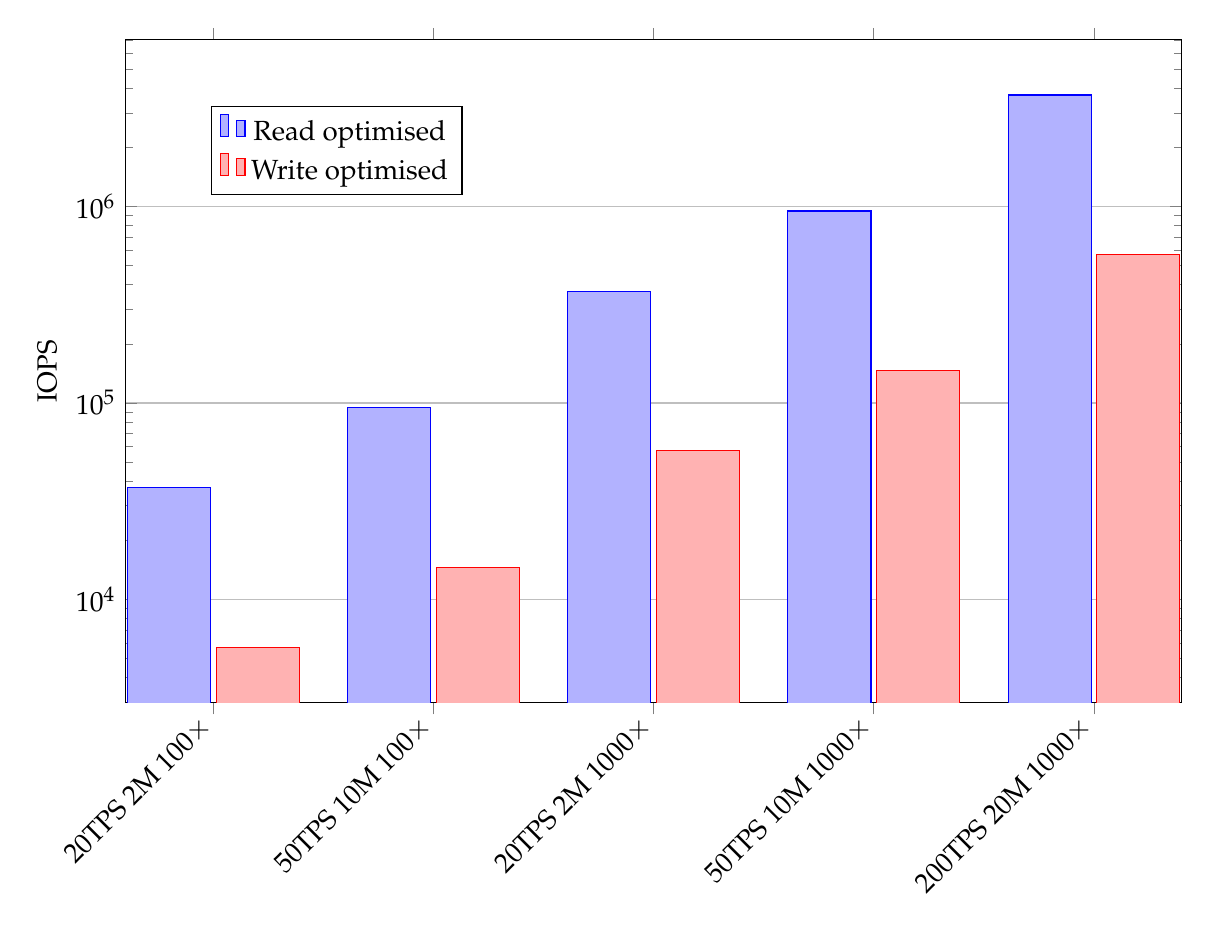
\begin{tikzpicture}
\begin{semilogyaxis} [
  ybar,
  ylabel = IOPS,
  ymajorgrids = true,
  bar width=30pt,
  %nodes near coords,
  symbolic x coords={20TPS 2M $100\times$,
                     50TPS 10M $100\times$,
                     20TPS 2M $1000\times$,
                     50TPS 10M $1000\times$,
                    200TPS 20M $1000\times$},
  xtick=data,
  x tick label style={rotate=45,anchor=east},
  legend style={at={(0.2,0.9)}, anchor=north},
  width = 15cm,
  height = 10cm,
]
\addplot coordinates {
    (20TPS 2M $100\times$,  37.0e3)
    (50TPS 10M $100\times$, 95.0e3)
    (20TPS 2M $1000\times$, 370.0e3)
    (50TPS 10M $1000\times$, 949.3e3)
    (200TPS 20M $1000\times$, 3699.0e3)
  };
\addplot coordinates {
    (20TPS 2M $100\times$,  5.7e3)
    (50TPS 10M $100\times$, 14.6e3)
    (20TPS 2M $1000\times$, 57.1e3)
    (50TPS 10M $1000\times$, 145.6e3)
    (200TPS 20M $1000\times$, 571.1e3)
   };
\legend{\strut Read optimised, \strut Write optimised}
\end{semilogyaxis}
\end{tikzpicture}
\caption{I/O performance feasibility for a read and write-optimised data store}
\label{fig:io-perf-feasibility}
\end{figure}

Some explanation of \cref{table:io-perf-feasibility-write,table:io-perf-feasibility-read} is in order:
\begin{itemize}
\item The first three columns are the targets for TPS, number of stake
      addresses and synchronisation speed. We use the threshold, middle and
      stretch targets for TPS (20, 50 and 200), and for stake addresses (2M,
      10M, 20M) and we use the threshold and stretch targets for
      synchronisation speed (100$\times$ and 1000$\times$).
\item The IOPS column is the number of I/O operations per second required to be
      able to meet the given combination of targets. These values are the
      result of evaluating \cref{eq:iops-read-optimised,eq:iops-write-optimised}
      for the given combination of targets.
\item The final three columns indicate whether the required IOPS are within the
      capabilities of the hardware, for three capability levels:
      \begin{itemize}
      \item ~~10k IOPS: the minimum hardware requirement when using serial I/O.
      \item 100k IOPS: the minimum hardware requirement when using parallel I/O.
      \item ~~1M IOPS: the capability of state-of-the-art high end SSDs.
      \end{itemize}
\item Note that the last column is well beyond our minimum hardware
      requirements from \cref{table:disk-iops-constraints} -- indeed $10\times$
      beyond -- but it gives an indication of the headroom to scale with future
      or server-class hardware.
\end{itemize}

An alternative presentation of the same data is given in \cref{fig:io-perf-feasibility}. Note in particular that this uses a log axis. Coincidentally the
hardware IOPS limits we are interested in correspond to the log axis major grid
lines of $10^4$, $10^5$ and $10^6$ respectively, so it is straightforward to
see how the IOPS required compares to the IOPS available.

\subsection{SSD performance}
\label{ssd-performance}

To assess feasibility we need a sense of typical SSD performance. This is also
needed to assess if the minimum hardware requirements (from
\cref{table:disk-iops-constraints}) are reasonable.

In addition to SSDs, we will include the performance of spinning disks but only
to illustrate that their performance is so poor as to be out of the question.

To make things concrete we look at the example of Samsung SSDs. Samsung
manufacture a range of medium to high performance consumer and server SSDs. They
helpfully publish rated performance numbers including low and high queue depth.
We select a vaguely representative sample of their range, picking 500GB models
where possible. For our spinning disk comparison we select a couple models from
Western Digital. Western Digital do not consistently publish performance numbers
for their disk drives, so some numbers below are taken from 3rd party reviews,
or are omitted entirely.
\begin{center}
\begin{tabular}[]{llll}
  Model & Capacity & Interface type & Comment \\
  \toprule
  WD Blue      & 1TB   & SATA        & Mainstream, low cost spinning disk \\
  WD Black     & 1TB   & SATA        & `High performance' spinning disk  \\
  \midrule
  870 QVO      & 1TB   & SATA        & Latest gen, high capacity, lower performance \\
  860 PRO      & 512GB & SATA        & Previous gen high performance SATA \\
  960 EVO      & 512GB & NVMe PCIe 3 & Previous gen high performance NVMe \\
  970 EVO Plus & 500GB & NVMe PCIe 3 & Current gen high performance NVMe \\
  980 PRO      & 500GB & NVMe PCIe 4 & Current gen ultra-high performance NVMe
\end{tabular}
\end{center}
The random read performance is given at ``queue depth 1'' and at ``queue depth
32''. Queue depth 1 means issuing all I/O operations serially, whereas a high
queue depth implies continuously issuing many I/O operations in parallel, so
that the hardware it given 32 operations to do at any one time.
\begin{center}
\begin{tabular}[]{lrrr}
  Model & 4k reads at QD1 & 4k reads at QD32 & QD32 speedup \\
  \toprule
  WD Blue      &    --       &     128 IOPS & -- \\
  WB Black     &    200 IOPS &     500 IOPS & $2.5\times$ \\
  \midrule
  870 QVO      & 11,000 IOPS &  98,000 IOPS & $9\times$ \\
  860 PRO      & 11,000 IOPS & 100,000 IOPS & $9\times$ \\
  960 EVO      & 14,000 IOPS & 330,000 IOPS & $23\times$ \\
  970 EVO Plus & 19,000 IOPS & 480,000 IOPS & $25\times$ \\
  980 PRO      & 22,000 IOPS & 800,000 IOPS & $35\times$
\end{tabular}
\end{center}
On the write side, some on-disk data structures are sensitive to random writes,
while others rely on sequential writes. The WD Blue model is omitted as the
numbers are not readily available.
\begin{center}
\begin{tabular}[]{lrrr}
  Model & 4k writes at QD1 & 4k writes at QD32 & sequential writes \\
  \toprule
  WB Black     &    450 IOPS &       460 IOPS &   176 MB/s \\
  \midrule
  870 QVO      & 35,000 IOPS &    88,000 IOPS &   530 MB/s \\
  860 PRO      & 43,000 IOPS &    90,000 IOPS &   530 MB/s \\
  960 EVO      & 50,000 IOPS &   330,000 IOPS & 1,800 MB/s \\
  970 EVO Plus & 60,000 IOPS &   550,000 IOPS & 3,200 MB/s \\
  980 PRO      & 60,000 IOPS & 1,000,000 IOPS & 5,000 MB/s
\end{tabular}
\end{center}
There are a number of things to note:
\begin{itemize}
\item Many of these are relatively high end and expensive SSDs (which in turn
      require relatively high performance and expensive desktop or server
      platforms). Minimum system requirements can only be at the lower end of
      this range.
\item There is huge difference between serial and parallel performance:
      typically a factor of 10 to 20 times.
\item Read performance at queue depth 1 has only slightly improved over time.
\item Read performance at high queue depths continues to improve from one
      generation to the next.
\item Sequential write performance is even higher than random 4k writes at
      high queue depth, typically by an extra 40--50\%.
\item Spinning hard drives have extremely low random access performance, though
      moderate sequential performance.
\end{itemize}
Real world performance numbers are less than the manufacturer rated numbers,
once practical details like file systems and OS I/O APIs are taken into account.
The author has benchmarked a Samsung 960 EVO 250GB model under Linux using the
ext4 file system on an encrypted block device, using the {\tt fio} benchmarking
tool. While rated by the manufacturer at 330k IOPS for random reads at QD32,
the {\tt fio} benchmark shows that at QD32 it achieves around 220k IOPS.

In conclusion, the minimum hardware requirement from
\cref{table:disk-iops-constraints} are reasonable. They are at the lower end
of the current generation of SSDs.


\subsection{AWS cost of memory vs. IOPS}

Most SPOs run their nodes using cloud VM instances or rented physical machines.
Not all such instances have access to high IOPS SSDs, so the question arises:
is it cheaper to use RAM to keep data in memory, or cheaper to use high IOPS
and keep data on disk. We will look at this question in the context of AWS
as it is one of the major providers of cloud VMs.

AWS provides hundreds of different types of VM instance, all with different
characteristics and price. These instance types provide two main kinds of disk
access: all instances support networked EBS volumes, and some have local SSDs
(of which some are NVMe while others are older technology). AWS publishes IOPS
figures for EBS volumes but not for local SSDs -- presumably because it depends
on the OS the user chooses. We have not benchmarked any AWS instances for this
report but we will assume that the local SSDs marketed as ``NVMe'' will achieve
over 100k IOPS, while we will assume the non-NVMe SSDs achieve less than 100k
IOPS -- as they are presumably SATA drives.

The cost of EBS volumes with high IOPS is very significant. The cheapest EBS
option is the `gp2' volume type, but it tops out at 16k IOPS. The high
performance option is the `io2' volume type which can provision higher IOPS,
but at significant cost. The table below is the current cost for these two
EBS volume types.
\begin{center}
\begin{tabular}[]{rrr}
           & EBS `gp2' \$/month & EBS `io2' \$/month \\
  \toprule
 128 GB storage & \$ 10 & \$ 16 \\
  \midrule
   3k IOPS & \$  0 & \$   195 \\
  16k IOPS & \$ 80 & \$ 1,040 \\
  32k IOPS & ---           & \$ 2,080 \\
  64k IOPS & ---           & \$ 3,552 \\
 128k IOPS & ---           & \$ 5,600 \\
\end{tabular}
\end{center}
By contrast, the cost of AWS instance types with small local SSDs is not
significantly more than equivalent EBS-only instances, though the choice of
instances with local SSDs is limited. To answer the question of cost of memory
vs disk, we should look at the instance types with the cheapest memory, and the
cheapest\footnote{There are hundreds of AWS instance types, with new ones added
frequently so it is hard to be sure that the examples chosen are the cheapest
available. Consider them as indicative.} instance types with local NVMe SSDs:
\begin{center}
\begin{tabular}[]{lrrrrr}
AWS instance & Arch & vCPUs & RAM & Local SSD storage & \$/month \\
\toprule
x2gd.large  & Arm    & 2 & 32 GiB & 118 GiB NVMe & \$120.24 \\
x2gd.xlarge & Arm    & 4 & 64 GiB & 237 GiB NVMe & \$240.48 \\
r6a.xlarge  & x86-64 & 4 & 32 GiB & EBS Only     & \$163.30 \\
r6a.2xlarge & x86-64 & 8 & 64 GiB & EBS Only     & \$326.59 \\
\midrule
m6gd.medium & Arm    & 1 &  4 GiB &  59 GiB NVMe & \$32.54 \\
m6gd.large  & Arm    & 2 &  8 GiB & 118 GiB NVMe & \$65.09 \\
m5ad.large  & x86-64 & 2 &  8 GiB &  75 GiB NVMe & \$74.16
\end{tabular}
\end{center}
The first group of instances are the `cheap memory' ones, assuming the ledger
state will fit within 32 or 64 GiB, while the second group are the `cheap local
SSD' options. It is clear that the cheaper option is storing the data on disk
than in memory.

Note that each of these instances would also need an EBS volume for non-ledger
storage, but these could be the cheaper `gp2' volumes, without special IOPS
requirements. Note that the Arm based instance types are cheaper, but it
will take some more time before the node can be fully validated on Arm. So
these are indicative of future lower cost options.

\subsection{The need for a write-optimised backend}

It is clear from
\cref{table:io-perf-feasibility-write,table:io-perf-feasibility-read,fig:io-perf-feasibility} that a write-optimised disk data structure is necessary to achieve
most of the performance targets. Given the write-heavy workload of the UTxO
table, it is not surprising that a write-optimised disk data structure will
perform better, but the numbers make clear that (when synchronising)
this performance advantage is necessary to fit within the hardware constraints.

The original report, \cite{utxo-db} Section 8, discusses the primary choices of
on-disk data structure: B+ trees (such as LMDB) which are not write-optimised,
and LSM trees which are write-optimised. It recommends an initial integration
with an existing B+ tree implementation, and recommends an LSM tree
implementation to meet the performance targets in the longer term. The original
analysis remains valid. A write-optimised disk data structure is necessary to
achieve more than the threshold performance targets, and an LSM is a good
choice for such a data structure.

\subsection{The need for parallel I/O}

It is also clear from
\cref{table:io-perf-feasibility-write,table:io-perf-feasibility-read,fig:io-perf-feasibility} that using parallel I/O is necessary to achieve more than the
threshold targets.

The implication for the project is that disk backends, such as LMDB, that use
only serial I/O cannot achieve more than the threshold targets, and that to
achieve the middle or stretch targets requires a disk backend that can use
parallel I/O to effectively take advantage of modern SSDs. Furthermore, a disk
backend using parallel I/O effectively may be able to hit the stretch targets,
but only when used with higher performance SSD hardware.

This is the same conclusion of the original report, see \cite{utxo-db} Sections
5.7, 6.1, 8.1, 8.3 and 9.

\subsection{The need for monoidal updates}

As discussed in \cref{sec:maintaining-the-stake-distribution-by-stake-address},
the operations the ledger needs to perform could make good use of an
{\sc update} operation, and some write-optimised disk data structures can
support {\sc update} more efficiently than the combination of a {\sc lookup}
and {\sc insert}.

The question is if this feature is necessary to achieve performance targets.
The answer is yes it is necessary, and we can use our quantitative method to
demonstrate it.

Recall that starting with \cref{eq:total-ops-1,eq:total-ops-2} we derived the
IOPS cost for the write-optimised case, as \cref{eq:iops-write-optimised}:
\begin{equation*}
\mathit{sync} \left(
    2.8 \; \mathit{tps} + \frac{0.24 |stake|}{\mathit{epochsec}}
  \right)\quad\text{IOPS}
\end{equation*}
This derivation was based on the assumption from
\cref{eq:io-ops-write-optimised} that the {\sc update} would cost 0.1 IOPS. If
we assume instead that {\sc update} costs the same as a {\sc lookup} plus an
{\sc insert} then it will cost 1.1 IOPS. With this assumption we would derive
the total IOPS cost to be
\begin{equation*}
\mathit{sync} \left(
    6.8 \; \mathit{tps} + \frac{1.24 |stake|}{\mathit{epochsec}}
  \right)\quad\text{IOPS}
\end{equation*}

Evaluating these and comparing them in \cref{fig:io-perf-update-op}, we can see
that the lack of an efficient {\sc update} not only makes a significant
difference, but it makes the difference between hitting or missing targets.
Note again that this uses a log axis, so the modest visual differences are
large numeric differences.

\begin{figure}
\centering
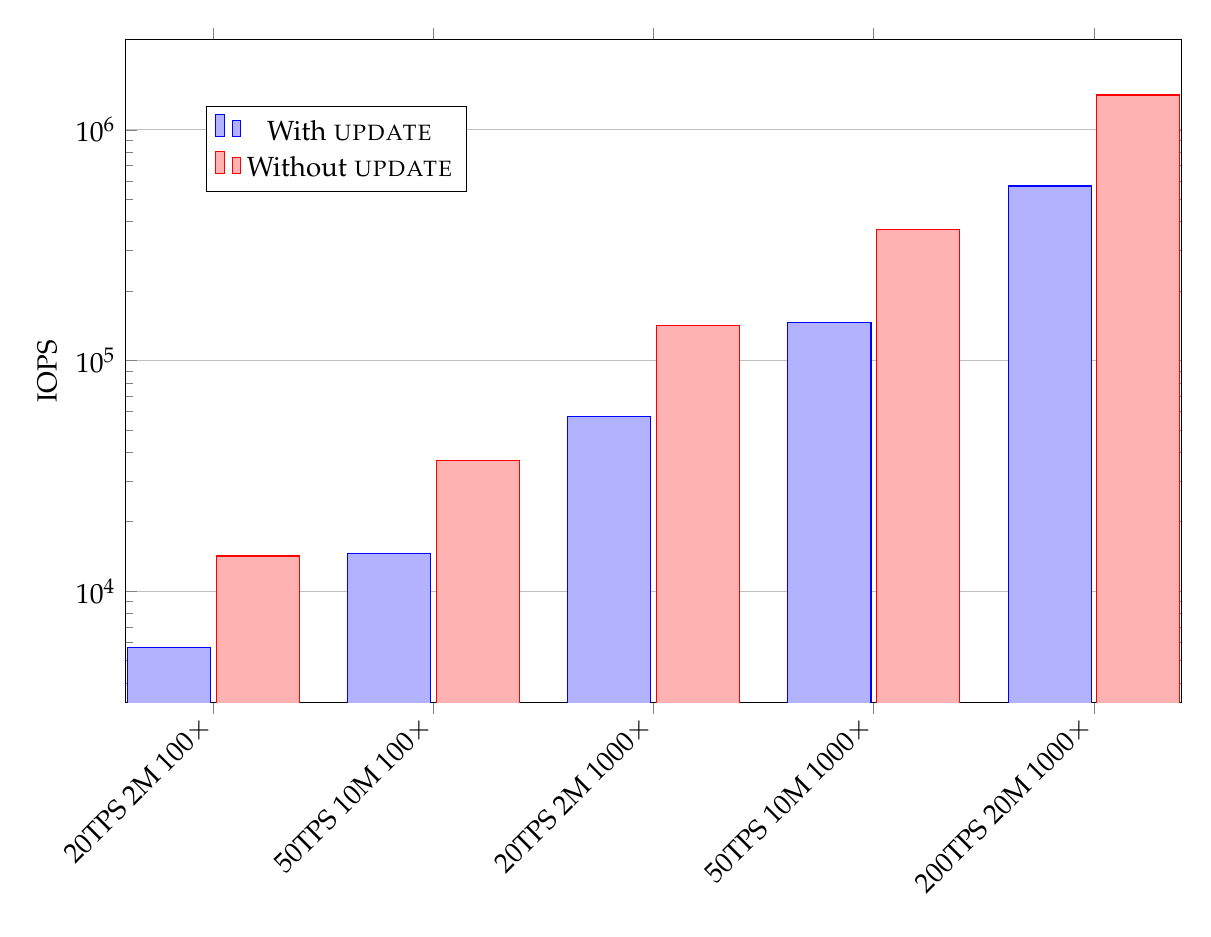
\begin{tikzpicture}
\begin{semilogyaxis} [
  ybar,
  ylabel = IOPS,
  ymajorgrids = true,
  bar width=30pt,
  %nodes near coords,
  symbolic x coords={20TPS 2M $100\times$,
                     50TPS 10M $100\times$,
                     20TPS 2M $1000\times$,
                     50TPS 10M $1000\times$,
                    200TPS 20M $1000\times$},
  xtick=data,
  x tick label style={rotate=45,anchor=east},
  legend style={at={(0.2,0.9)}, anchor=north},
  width = 15cm,
  height = 10cm,
]
\addplot coordinates {
    (20TPS 2M $100\times$,  5.7e3)
    (50TPS 10M $100\times$, 14.6e3)
    (20TPS 2M $1000\times$, 57.1e3)
    (50TPS 10M $1000\times$, 145.6e3)
    (200TPS 20M $1000\times$, 571.1e3)
  };
\addplot coordinates {
    (20TPS 2M $100\times$,  14.2e3)
    (50TPS 10M $100\times$, 36.9e3)
    (20TPS 2M $1000\times$, 141.7e3)
    (50TPS 10M $1000\times$, 368.7e3)
    (200TPS 20M $1000\times$, 1417.4e3)
  };
\legend{\strut With {\sc update}, Without {\sc update}}
\end{semilogyaxis}
\end{tikzpicture}
\caption{I/O performance with and without an efficient {\sc update} operation}
\label{fig:io-perf-update-op}
\end{figure}

\subsection{The need for other special operations}

The existing MVP design makes use of a {\sc snapshot} operation, used as part
of checkpointing the whole chain and ledger state. The full design with all the
stake related tables will have additional uses for the {\sc snapshot} operation,
and additional timing constraints. We established in \cref{sec:table-snapshots}
that the {\sc snapshot} operation must have $\mathcal{O}(\log n)$ cost because
any higher cost would cause unacceptable stalls in the operation of the system.

In \cref{sec:updating-stake-rewards} we discussed the hard problem of updating
the reward account balances at the epoch boundary without causing stalls. The
best design idea we have is to require a {\sc merge} operation, which must have
at most $\mathcal{O}(\log n)$ cost to avoid unacceptable stalls.

\subsection{Infeasibility of using the existing LMDB backend}
\label{sec:performance-limits-of-the-lmdb-backend}

We have established that to meet performance targets, we need:
\begin{itemize}
\item a write-optimised data store,
\item good support for parallel I/O,
\item support for monoidal updates,
\item support for an $\mathcal{O}(\log n)$ {\sc snapshot} operation, and
\item support for an $\mathcal{O}(\log n)$ {\sc merge} operations.
\end{itemize}
The LMDB backend has \emph{none} of these characteristics, and is thus not a
suitable choice.

Note that in principle, the LMDB library has some support for parallel I/O via
its support for concurrent clients operating on independent transactions.
Unfortunately this does not fit well with our use case of a single client that
wants to perform batches of lookups in parallel. The backend using LMDB could
be adapted to use multiple OS threads with an LMDB transaction for each thread
and to perform lookups from each thread, but at quite a high implementation
complexity cost. This would scale I/O performance to some degree but the
overheads of spreading out the requests and collecting the results from the
many threads would limit the improvement. The overheads would be proportionally
worse for SSDs with higher IOPS, since the overhead per operation is fixed.

It may be helpful to get an intuition of why the LMDB backend was a suitable
choice for a MVP, but cannot be a suitable choice for a full implementation
that meets the performance targets from the business requirements.

The size of the UTxO is currently well below the minimum target. Furthermore,
the node process is being run on host machines that have plenty of RAM. This
combination means that the disk files that make up the UTxO table can be kept
wholly in RAM (in the OS page cache), and thus no I/O is needed to perform
lookups. The use of the OS page cache does not show up in the measurement of
the memory used by the node process, but it is essential for the current good
I/O performance. As the UTxO grows, or if the node is run on a machine with
less memory, then inevitably the UTxO will no longer fit into the page cache.
At this point, the I/O bottleneck will limit performance, as discussed earlier
in this section. In particular, the LMDB backend will be limited to the serial
I/O limit of SSDs, unless it can be modified to partially take advantage of parallel I/O as described above.

In summary, the LMDB backend can meet the current needs of the chain only
because those current needs are well below the minimum targets from the
business requirements.

\subsection{Table operations and IOPS for other alternative design choices}

We have already looked at whether we need a write-optimised design, parallel
I/O, and monoidal updates -- and it turns out that we need all of them! There
are some other design decisions we have mentioned in previous sections that we
can evaluate in the same quantitative manner.

\subsubsection{Maintaining the stake distribution by stake address}

In \cref{sec:maintaining-the-stake-distribution-by-stake-address} we considered
two methods of maintaining the stake distribution by stake address: the
continuous or bulk method. The continuous method involves one {\sc update}
operation for each transaction input and output.
\begin{equation}
\begin{aligned}
      & |\mathit{txin}| \; \text{{\sc update}}_\text{stake} \\
 + \; & |\mathit{txout}| \; \text{{\sc update}}_\text{stake} \\
\end{aligned}
\end{equation}
The bulk method involves a linear scan of the UTxO snapshot, accumulating and
aggregating into a target table keyed on the stake credential.
\begin{equation}
\begin{aligned}
      & \text{{\sc snapshot}}_\text{utxo} \\
 + \; & \frac{1}{\mathit{epochsec}}\text{{\sc scan}}_\text{stake} \\
 + \; & \frac{|\mathit{stake}|}{\mathit{epochsec}} \; \text{{\sc update}}_\text{stake} \\
\end{aligned}
\end{equation}
Using these as modifications to the overall operation counts, and then using
the I/O cost for a write-optimised design we can re-derive the cost in IOPS.
The continuous method is our default design option so we get the same formula
as \cref{eq:iops-write-optimised}
\begin{equation*}
\mathit{sync} \left(
    2.8 \; \mathit{tps} + \frac{0.24 |stake|}{\mathit{epochsec}}
  \right)\quad\text{IOPS}
\end{equation*}
or for the bulk method we get
\begin{equation*}
\mathit{sync} \left(
    2.4 \; \mathit{tps} + \frac{0.375 |stake|}{\mathit{epochsec}}
  \right)\quad\text{IOPS}
\end{equation*}
As we would expect, this has a lower factor for TPS but a higher factor for
the number of stake addresses.

Evaluating these and comparing them in \cref{fig:io-perf-stake-by-addr}, we see
that the bulk method does result in fewer IOPS, but that overall the difference
is not very significant. It seems reasonable therefore to decide on the basis
of code complexity rather than IOPS cost.

\begin{figure}
\centering
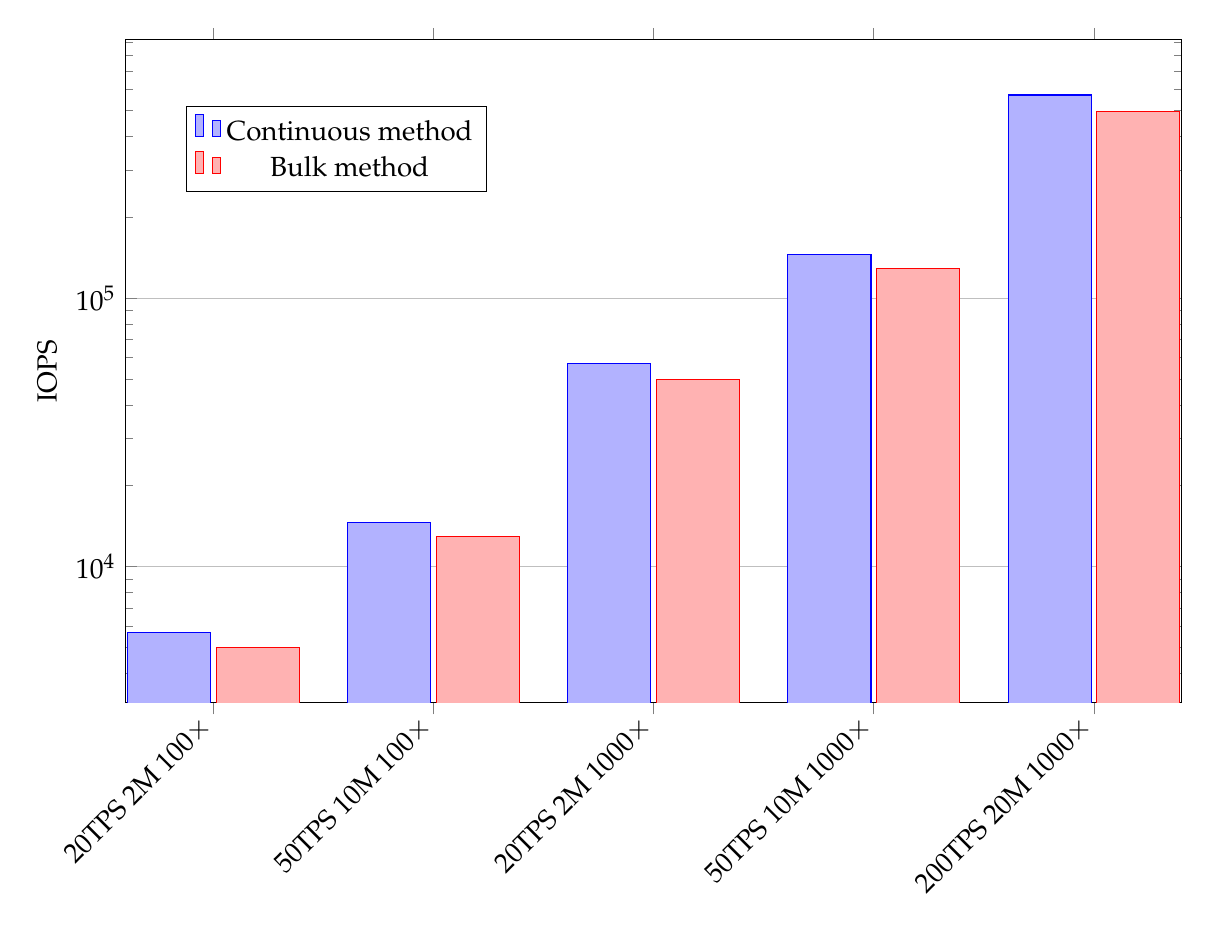
\begin{tikzpicture}
\begin{semilogyaxis} [
  ybar,
  ylabel = IOPS,
  ymajorgrids = true,
  bar width=30pt,
  %nodes near coords,
  symbolic x coords={20TPS 2M $100\times$,
                     50TPS 10M $100\times$,
                     20TPS 2M $1000\times$,
                     50TPS 10M $1000\times$,
                    200TPS 20M $1000\times$},
  xtick=data,
  x tick label style={rotate=45,anchor=east},
  legend style={at={(0.2,0.9)}, anchor=north},
  width = 15cm,
  height = 10cm,
]
\addplot coordinates {
    (20TPS 2M $100\times$,  5.7e3)
    (50TPS 10M $100\times$, 14.6e3)
    (20TPS 2M $1000\times$, 57.1e3)
    (50TPS 10M $1000\times$, 145.6e3)
    (200TPS 20M $1000\times$, 571.1e3)
  };
  4973.611111111111,
  12868.055555555555,
  49736.11111111111,
  49736.11111111112,
  128680.55555555555,
  497361.11111111107
\addplot coordinates {
    (20TPS 2M $100\times$,  5.0e3)
    (50TPS 10M $100\times$, 12.9e3)
    (20TPS 2M $1000\times$, 49.7e3)
    (50TPS 10M $1000\times$, 128.6e3)
    (200TPS 20M $1000\times$, 497.4e3)
  };
\legend{\strut Continuous method, Bulk method}
\end{semilogyaxis}
\end{tikzpicture}
\caption{I/O performance for methods of maintaining the stake distribution by stake address}
\label{fig:io-perf-stake-by-addr}
\end{figure}

\subsubsection{Maintaining the stake distribution by stake pool or DRep}

In \cref{sec:maintaining-the-stake-distribution-by-stake-pool-or-DRep} we
considered two methods of maintaining the stake distribution by stake pool (or
equivalently by DRep): the continuous or bulk method. The continuous method
would extend the continuous method for maintaining the stake distribution by
stake address: where additionally each input and output stake credential must
be looked up in the mapping of stake credential to delegation choice. Counting
only the additional operations, this gives us
\begin{equation}
\begin{aligned}
      & |\mathit{txin}| \; \text{{\sc lookup}}_\text{stake} \\
 + \; & |\mathit{txout}| \; \text{{\sc lookup}}_\text{stake} \\
\end{aligned}
\end{equation}
The bulk method involves a scan of the mapping of stake credential to stake and
of the mapping of stake credential to delegation choice.
\begin{equation}
      \frac{2}{\mathit{epochsec}} \; \text{{\sc scan}}_\text{stake} \\
\end{equation}
Using these as modifications to the overall operation counts, and then using
the I/O cost for a write-optimised design we can re-derive the cost in IOPS.
For the continuous method we get
\begin{equation*}
\mathit{sync} \left(
    6.8 \; \mathit{tps} + \frac{0.17 |stake|}{\mathit{epochsec}}
  \right)\quad\text{IOPS}
\end{equation*}
while bulk method is our default design option so we get the same formula
as \cref{eq:iops-write-optimised}
\begin{equation*}
\mathit{sync} \left(
    2.8 \; \mathit{tps} + \frac{0.24 |stake|}{\mathit{epochsec}}
  \right)\quad\text{IOPS}
\end{equation*}
As we would expect, the continuous method has a higher factor for TPS but a
lower factor for the number of stake addresses.

Evaluating these and comparing them in \cref{fig:io-perf-stake-distr}, we see
that the continuous method is substantially more expensive, and indeed
sufficiently more expensive to make it infeasible to meet several of the
targets. Note again that this uses a log axis, so the modest visual differences
are large numeric differences.

\begin{figure}
\centering
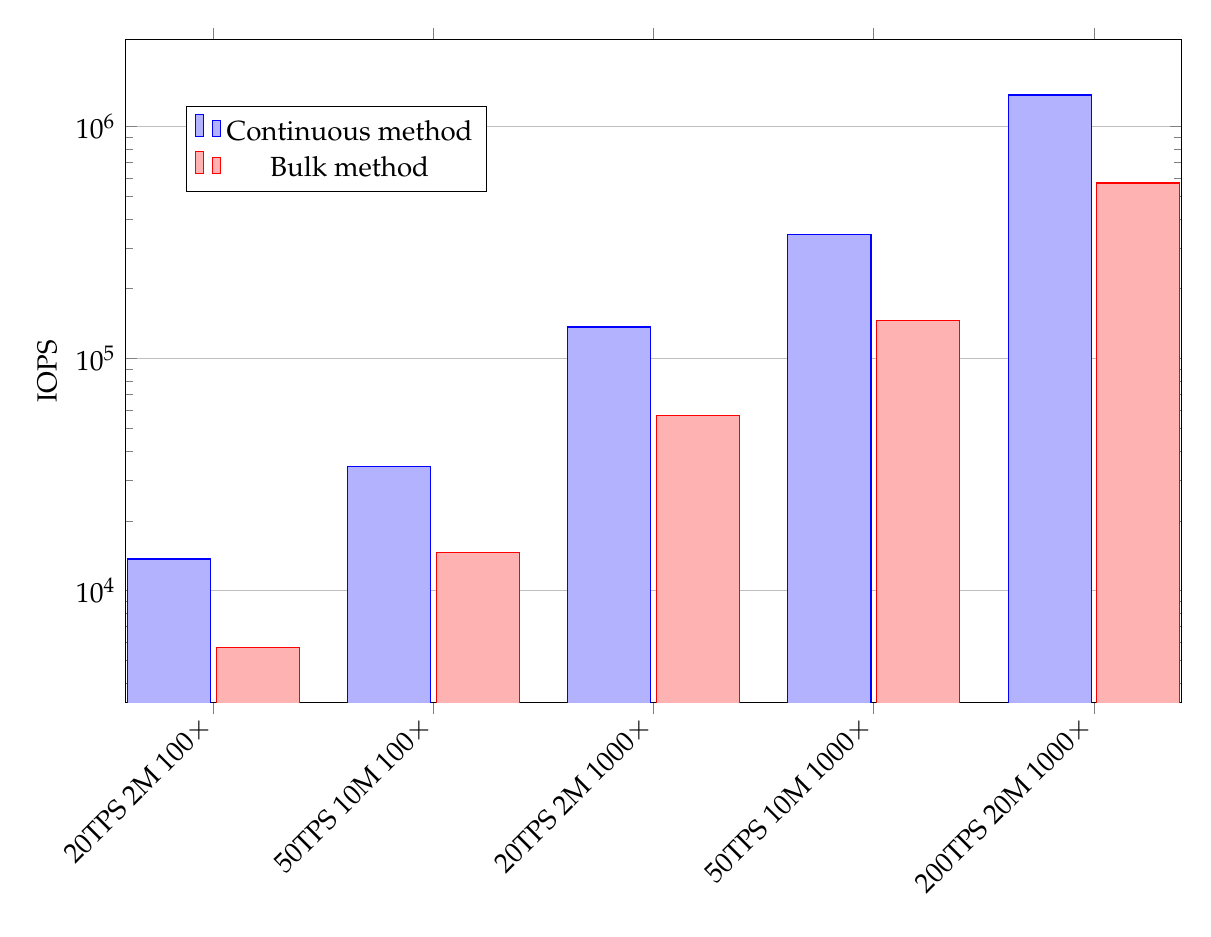
\begin{tikzpicture}
\begin{semilogyaxis} [
  ybar,
  ylabel = IOPS,
  ymajorgrids = true,
  bar width=30pt,
  %nodes near coords,
  symbolic x coords={20TPS 2M $100\times$,
                     50TPS 10M $100\times$,
                     20TPS 2M $1000\times$,
                     50TPS 10M $1000\times$,
                    200TPS 20M $1000\times$},
  xtick=data,
  x tick label style={rotate=45,anchor=east},
  legend style={at={(0.2,0.9)}, anchor=north},
  width = 15cm,
  height = 10cm,
]
\addplot coordinates {
    (20TPS 2M $100\times$,  13.7e3)
    (50TPS 10M $100\times$, 34.4e3)
    (20TPS 2M $1000\times$, 136.8e3)
    (50TPS 10M $1000\times$, 343.9e3)
    (200TPS 20M $1000\times$, 1367.9e3)
  };
\addplot coordinates {
    (20TPS 2M $100\times$,  5.7e3)
    (50TPS 10M $100\times$, 14.6e3)
    (20TPS 2M $1000\times$, 57.1e3)
    (50TPS 10M $1000\times$, 145.6e3)
    (200TPS 20M $1000\times$, 571.1e3)
  };
\legend{\strut Continuous method, Bulk method}
\end{semilogyaxis}
\end{tikzpicture}
\caption{I/O performance for methods of maintaining the stake distribution by DRep}
\label{fig:io-perf-stake-distr}
\end{figure}

\section{Assuring node robustness in the presence of I/O faults}
\label{sec:assurance}

\subsection{The importance of I/O fault testing}

Disk I/O errors can and do happen, e.g. due to hardware failures, or power
outages. They are not the fault of the code itself, but are an aspect of the
environment in which the code runs. Testing for correct behaviour in the
presence of I/O faults is notoriously difficult. Such I/O faults happen rarely
in practice, so I/O fault testing is usually based on fault simulation or
injection.

The benefit of the I/O fault testing should not be underestimated. The original
Cardano node deployed at the original Byron Genesis suffered from occasional
disk or database corruption which could not be reproduced or diagnosed by the
development team, but occurred sufficiently frequently in production with users
and exchanges that it created a substantial workload for the support team, and
contributed to a poor reputation. In the Shelley re-design, the issue of
robustness in the presence of I/O faults and disk corruption was taken
seriously. The solution in the Shelley re-design was to develop and use a test
framework that can simulate I/O errors and silent disk corruption and check
that the node can detect and recover from them. This has proved very successful
in practice: such errors and complaints are now almost unheard of and they no
longer generate a significant load for the support team.

The I/O fault testing framework however relies on the code under test
interacting with the filesystem \emph{only} via a specific API that is provided by the Haskell-based I/O simulation framework. In practice this means it must
be written in Haskell\footnote{While it is plausible to imagine a C library for
disk data structures that only interact with the filesystem via a callback
interface that could be implemented by Haskell test code on top of a mock
filesystem, in practice production C database libraries are not written in this
way.}. The three original Shelley on-disk components (immutable DB, volatile DB
and ledger DB) were all written in the appropriate style (using the simulation
framework's filesystem API) to be used with the simulation and I/O fault testing
framework. The LMDB backend however relies on the LMDB C library which cannot
be practically adjusted to run within the I/O simulation or to use the required
filesystem API. Thus overall, when using this backend it is no longer possible
to use I/O fault testing for the consensus layer as a whole.

This is the motivation for using an on-disk backend that is written in Haskell,
and that uses the consensus's existing I/O simulation and I/O fault testing
framework.

\subsection{How to test disk components are robust against I/O faults}
\label{sec:how-to-test-disk-components-are-robust-against-io-faults}

The basic requirement is that all disk components use the \texttt{io-sim}
library to allow running in simulation and do all their I/O via the
\texttt{fs-sim} library API. This allows running the component in simulation
with a simulated file system, and allows for the I/O fault injection.

There are two main kinds of I/O fault: `noisy' and `silent'. The noisy faults
are ones which are reported synchronously, usually as I/O exceptions, such as
failure to write to a file or the disk being full. This could also include
data corruption detected as part of a read operation (e.g. checking a checksum
after reading data). The silent faults are those that do not report a problem
at the time the problem occurs, but results in data being lots or corrupted.
A primary example is data failing to be persisted to disk due to the machine
being turned off, but this could also include undetected hardware faults and
bit flips due to cosmic rays.

Running in simulation is necessary but not sufficient. We want to establish
some robustness properties. The general property for the consensus layer
overall is to treat I/O faults as a truncation of the blockchain. Truncation is
obviously not desirable, but it is acceptable if it is infrequent (and not
correlated with external events).

The general strategy taken by the consensus layer is to detect errors and upon
detecting an error, to shutdown and restart the node. Upon restarting, the
strategy is to check carefully for file corruption errors. If any are found
then the disk state must be adjusted so that it is the equivalent of a
truncation of the blockchain. In particular for the ledger state, the consensus
layer strategy is to take occasional snapshots of the ledger state and on
startup to restore from the most recent non-corrupted snapshot. Any corrupted
snapshots are deleted. In the worst case this involves replaying from genesis.

It is generally not required nor useful to try to recover directly from
individual I/O faults.

Thus for the on-disk table component
\begin{itemize}
\item we need to be able to detect and report corruption found during
      restoration. Being able to detect corruption may require the use of
      checksums.
\item We need to report any `noisy' I/O faults during normal operation so that
      the consensus layer can shut down and restart the whole node.
\item It is not necessary to detect all silent corruption during normal
      operation. This is a trade-off: doing so would be expensive and this kind
      of corruption is rare. The most common kind of corruption is recently
      written data failing to make it to disk before the process or machine is
      terminated, and this kind can be detected on restoration.
\end{itemize}

\section{Integrating a new high performance disk backend}

A new disk backend that fits the existing interface should be possible to
integrate relatively easily -- at least for functional correctness. The
performance effects are more subtle.

The summary is that,
\begin{itemize}
\item for a drop-in replacement disk backend, the consensus layer would benefit
      from I/O \emph{batching} which provides a limited degree of I/O
      parallelism and a corresponding performance improvement; but
\item to achieve full I/O parallelism, the consensus layer would need to be
      adapted to take advantage of the pipelined style of the existing
      interface, to execute multiple batches of I/O reads \emph{concurrently}.
\end{itemize}

It is also important to distinguish the integration of a new backend from the
full exploitation of the new backend, either for performance or the use to
support moving the large stake-related tables to disk.

\subsection{Fitting the existing interfaces}
\label{sec:fitting-the-existing-interfaces}

The interface between the consensus and disk backends uses the `pipelined'
style that was originally recommended and prototyped. This was designed with
a high throughput backend in mind. It is therefore expected that a new high
throughput backend will be able to fit the existing interface with no changes
or minimal changes to the interface.

There are other aspects of integration that will require some work, including
\begin{itemize}
\item adjusting the code to initialise the new backend
\item integration testing
\item performance benchmarking
\item integrating with the I/O fault testing framework
\end{itemize}

The I/O fault testing framework interface will need some small adjustments.
The current I/O interface supported by the test simulation includes simple
blocking reads on single files. To support a new backend that can perform
parallel I/O will require a small extension. This is expected to be an extra
interface to perform batches of reads across multiple open files, but still as
a blocking operation overall. This should be straightforward to implement in
the simulator in terms of sequential operations and aggregation of any I/O
faults.

\subsection{Extending the existing interfaces for new operations}
\label{sec:extending-the-existing-interfaces-for-new-operations}

Part of the requirements for the new backend is new operations to support the
ledger when the stake-related tables are moved to disk. These were discussed in
detail in \cref{sec:requirements-for-storing-the-stake-related-tables-on-disk}.
In particular there is a new {\sc merge} operation and support for monoidal
updates. Exposing these new operations will require an extension to the
existing API between the backend and consensus layer. This should be a fairly
modest amount of work.

\subsection{Initial improvement to I/O parallelism by batching}

Once the new disk backend is integrated, the consensus layer will benefit from
improved I/O parallelism due to batching. This should work without significant
additional changes to the consensus layer. It should work with the existing
backend API, and the existing use of that API by the consensus layer.

The current design in the MVP is that all the transaction input lookups for all
the transactions in a whole block are submitted to the disk backend in a single
batch, followed by waiting for the results. A disk backend supporting parallel
I/O can take advantage of this batching to submit the reads in parallel. The
degree of parallelism is limited by the batch size. The batch size for the
consensus layer will be the number of inputs in each block.

The good thing about batching is that it is relatively straightforward to do
and to integrate. The performance benefits for reasonable sized batches should
be significant.

Batching alone cannot achieve full I/O utilisation however. This is due to the
fact that once one batch starts to complete, there is no more I/O work to do
for a while, and thus a lost opportunity to utilise the hardware. This is the
case even if batches are executed back-to-back sequentially. To fully utilise
the hardware, the next batch must be available to start, as soon as the SSD
hardware is ready to accept more I/O operations, which is \emph{before} the
previous operations fully completes. To utilise this fully requires pipelining.
See \cref{sec:a-possible-approach-to-io-pipelining-in-the-consensus-layer} for
details.

\section{Fully exploiting a new disk backend}

\subsection{Moving the stake related tables to disk}

The other half of the overall project is to move the remaining large parts of
the ledger state to disk. These are all the stake-related tables. Doing so will
take advantage of the new disk backend, in particular new operations and
improved performance of existing operations.

This part of the project will require substantial work in the consensus and
ledger layers. It will require several changes to the consensus/ledger
interface:
\begin{itemize}
\item changing to a multi-table design;
\item requiring the ledger state to be parameterised by the table type;
\item adding support for individual table snapshots;
\item adding support for read-only and monoidal table types;
\item adding support for table merges;
\end{itemize}
All but the last item above have been previously explored in the prototype,
prior to the MVP.

In the consensus layer it will require:
\begin{itemize}
\item introducing and using difference-tracking map types;
\item introducing and using difference-tracking monoidal map types;
\item tracking of snapshots within the `changelog';
\item routing reads via snapshots to the correct table.
\end{itemize}
In the ledger layer it will require:
\begin{itemize}
\item adapting to all the changes in the consensus/ledger interface;
\item moving each of the stake related tables to use the new consensus/ledger interface;
\item adapting the bulk incremental algorithms to use the new consensus/ledger interface;
\item converting any remaining bulk algorithms to be incremental;
\item using the new table merge operation for rewards payout;
\item functional testing;
\item performance testing, including verifying that there are no I/O related
      stalls at any point in the epoch.
\end{itemize}

\subsection{A possible approach to I/O pipelining in the consensus layer}
\label{sec:a-possible-approach-to-io-pipelining-in-the-consensus-layer}

Taking advantage of the pipelined style of the interface to the disk backend
will require design changes in the consensus layer. This is not necessary for
functional integration or for I/O batching, but would be needed to hit the
higher performance targets.

One possible design to incorporate pipelining into the existing consensus layer
would be to include it into the `chain db' component. The chain db already uses
an asynchronous approach to submitting new blocks: it has a queue of incoming
blocks for consideration for chain selection. It may be practical to adjust
this so that upon initial submission to the queue, the I/O reads for the block
are initiated, with the expectation that -- by the time the block is extracted
from the queue for validation -- the I/O reads have completed. The typical
length of the queue may need to be increased to give enough time for the I/O to
complete.

A challenge of this approach is that the chain db may need to track the pending
or completed reads for a block systematically throughout its volatile db
component. This is because blocks are not necessarily added to the chain as
soon as they are submitted to the chain db. For example, the chain db supports
blocks being submitted out of order (which can happen when blocks are
downloaded from multiple independent peers) which means the blocks will only be
added later once the `gaps' are filled.


\section{Opportunities with a new disk backend}
\label{sec:opportunities-with-a-new-disk-backend}

\subsection{Unusual requirements in the management of the ledger state}
\label{sec:unusual-requirements-in-the-management-of-the-ledger-state}

The consensus layer of Cardano node has some somewhat unusual requirements for
how it manages the ledger state -- which translates to unusual requirements for
storing the ledger state on-disk. These requirements arise from the Ouroboros
algorithm and the need to avoid denial of service (DoS) attacks.

Most applications that use databases only need a \emph{single} value of the
database to be available at once. This is not the case for the ledger state
managed by the consensus layer. The consensus layer needs many versions of the
ledger state to be available at once (with low cost) and it needs to be able to
extend (i.e. modify) any of these versions. This arises from the fact that the
node needs to be able to evaluate potential chain forks, and to avoid DoS
attacks it must be able to do so with reasonable cost.

\cite{fake-stake} (Section 3, "Attack on Disk") describe a class of potential
DoS attacks on PoS blockchains, such as Cardano. We believe our current
consensus design avoids this class of attack, but to do so it relies on being
able to cheaply obtain and extend the ledger state for any recent block, up to
$K$ (2160) blocks back.

In particular, evaluating an alternative chain fork works by first obtaining
evidence of a strictly longer chain of valid headers that intersects with the
current chain within the last $K$ blocks. Then the block bodies for this chain
are downloaded and verified. Verifying the blocks in the chain fork relies on
having access to the ledger state on the current chain at point where it
intersects with the fork. Then with the ledger state from the intersection
point, it must be extended as each block in turn on the fork is validated. Thus
not only is read access required for the recent ledger states, but any one of
them may need to be extended, without modifying the current ledger state (or
the state for any other fork being validated concurrently).

If each of these multiple ledger states were to be stored on disk then the
database would need to support multiple \emph{writable} snapshots. This is not
a feature that is available in most off-the-shelf database libraries, and not
available in the libraries that would otherwise be plausible choices for
Cardano. For example, LMDB and RocksDB support multiple read-only snapshots,
but not writable ones.

The need to use an off-the-shelf database library for the MVP necessitated a
somewhat complex and costly design. \cite{utxo-db-api} describes this design in
detail. The summary is that the consensus layer only keeps on disk the ledger
state corresponding to a block that is at least $K$ blocks old -- which is
therefore stable. The ledger states corresponding to all the more recent blocks
are maintained in memory using a representation of differences. This allows
keeping only a single copy of the ledger state on disk -- fitting within the
constraints of the LMDB library -- while still having access to all the
intermediate ledger states, and the ability to extend any one of them in memory.

\begin{center}
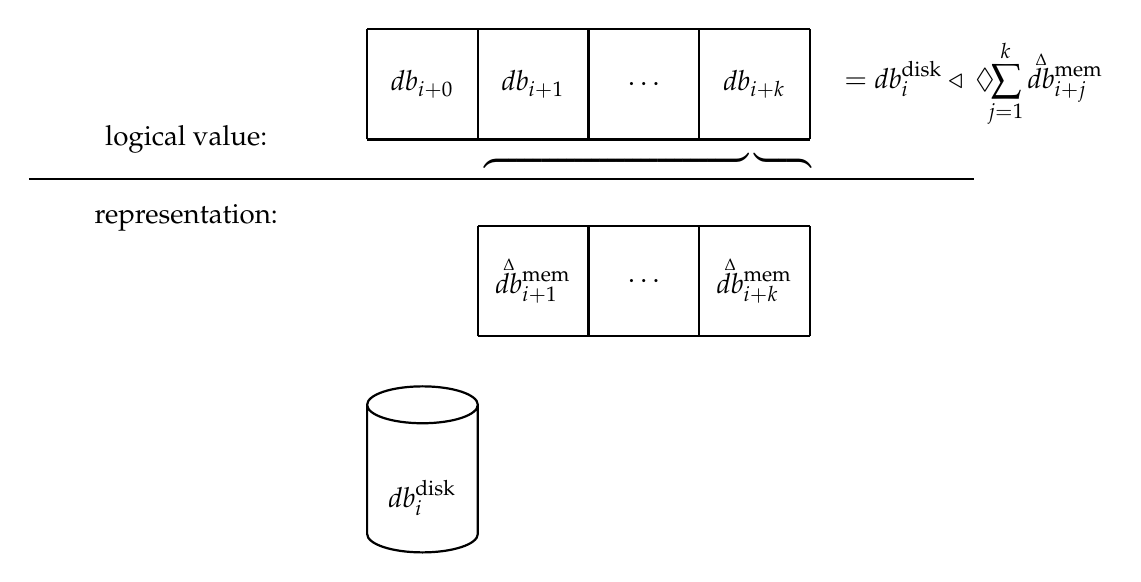
\begin{tikzpicture}[state/.style={circle, draw=black}]
\begin{scope}[thick]

  % disk icon
  \node[cylinder, aspect=2, rotate=90, draw, minimum height=60pt, minimum width=40pt]
        at (0,-25pt) {};
  \draw (0, -30pt) node {$\mathit{db}^{\mathrm{disk}}_i$};

  \begin{scope}[yshift=1cm, xshift=40pt]
  \draw[step=40pt,xshift=-20pt] (0,0) grid (120pt,40pt);
  \draw (0pt,  20pt) node {$\deltavar{\mathit{db}}^{\mathrm{mem}}_{i+1}$};
  \draw (40pt, 20pt) node {$\ldots$};
  \draw (80pt, 20pt) node {$\deltavar{\mathit{db}}^{\mathrm{mem}}_{i+k}$};
  \end{scope}

  % dividing line
  \draw (-5,3) -- (7,3);
  \draw (-3,3.5) node {logical value:};
  \draw (-3,2.5) node {representation:};

  % logical value
  \begin{scope}[yshift=3.5cm]
  \draw[step=40pt,xshift=-20pt] (0,0) grid (160pt,40pt);
  \draw (0,     20pt) node {$\mathit{db}_{i+0}$};
  \draw (40pt,  20pt) node {$\mathit{db}_{i+1}$};
  \draw (80pt,  20pt) node {$\ldots$};
  \draw (120pt, 20pt) node {$\mathit{db}_{i+k}$};
  \end{scope}

  \node [above delimiter=\rmoustache,
         xshift=70pt,yshift=2.9cm, minimum width=100pt] {};
  \node [above delimiter=\lmoustache,
         xshift=130pt,yshift=2.9cm, minimum width=20pt] {};

  \draw (7,3.5cm+20pt) node
        {$= \mathit{db}^{\mathrm{disk}}_i \triangleleft ~
            \displaystyle\Diamond\hspace{-4pt}\sum_{j=1}^k{\deltavar{\mathit{db}}^{\mathrm{mem}}_{i+j}}$};

\end{scope}
\end{tikzpicture}
\end{center}

This design has a complexity cost, and it also has a computational cost:
\begin{itemize}
\item The complexity cost translates into initial development time in the MVP
      and ongoing maintenance cost such as the time for new developers to
      become familiar with the codebase.
\item The performance regression between the prior in-memory design and the new
      in-memory test backend can be ascribed primarily to the extra costs of
      managing the sequence of differences. Work has already been carried out
      to minimise the cost of managing the sequence of differences\footnote{The
      improvement involved extending the operations on the representation of
      differences to make them a group rather than just a semi-group, which in
      turn allowed an improved algorithm for the key difference sequence
      maintenance operations which are now $\mathcal{O}(1)$ rather than
      $\mathcal{O}(\log n)$ in the length of the sequence (i.e. K).}, and
      further improvements are not expected.
\end{itemize}

\subsection{Opportunities to reduce code complexity}

If a new disk backend could directly support multiple writable versions of the
database on disk, and if it could do so with reasonable resource cost, then it
could enable a simpler consensus design that would eliminate the management of
explicit differences and their associated costs.

In the original in-memory design, the consensus layer directly keeps hold
of the whole ledger state for each of the last K blocks. This makes access to
old versions of the ledger state trivial. The representation uses persistent
data structures and thus shares the vast majority of the in-memory data between
all these versions. Indeed, one measurement for the mainnet found that the cost
of keeping $K$ versions was approximately 1\% higher than the cost of keeping a
single version. In theory the memory cost is directly related to the rate of
change (i.e. TPS) and how many copies are kept (i.e. $K$).

A disk backend supporting multiple writable versions of the database on disk
would allow a design analogous to the original design. The consensus layer
would keep hold of database references to the state corresponding to each of
the last K blocks. Then any of them are accessible and any can be extended
when a chain fork needs to be validated.

\subsection{Opportunities to reduce memory use}
\label{sec:opportunities-to-reduce-memory-use}

Furthermore, a new disk backend with support for multiple writable versions
could enable a design that uses less memory. In particular, while the design
for the MVP needs to keep track of all the differences in the last K blocks in
memory, the new design outlined above needs no such tracking of differences.

In the current MVP design, the size of the differences is proportional to the
data rate of the chain (which is proportional to block size), times the $K$
(2160) versions that the consensus layer needs access to. For the expected TPS
of the current Cardano implementation, this is an acceptable amount of memory.

For Leios however, the TPS is expected to be substantially higher and the
memory use would be correspondingly higher. A disk backend that supports
multiple writable versions could have a fixed memory use (for its write buffer)
rather than it being proportional to the blockchain TPS. This would translate
to a significant memory saving.

One must be careful however to account for memory used by the disk backend in
the proposed design, otherwise one may be simply shifting memory use from one
place to another. In particular, the new design calls for keeping K references
to versions of the database. We must account for the memory of these K
version references.

It is expected that a new disk backend will maintain a ``write buffer'' and
only flush data to disk when the write buffer is full. By bounding the buffer
size, the memory use can be bounded. However each version reference can be
expected to have its own write buffer. Even if the write buffer uses a
persistent data structure to share values between versions, if K versions are
kept then all changes in the last K versions will still have to be kept in
memory.

To avoid this, we can keep fewer versions, and make the buffers smaller.

\paragraph{Keeping fewer versions}
Keeping references to fewer versions is possible in principle and indeed an
earlier version of the consensus layer for Cardano Shelley did so. The
observation is that while we need to be able to get hold of the ledger state
for any of the last $K$ blocks, we do not need to store them all if we can
compute them within reasonable cost. The early Shelley design only kept the
ledger state for every ``n'th'' block. This feature was not kept because the
memory savings for the in-memory design were insignificant, but for an on-disk
design the savings could be considerable.

\paragraph{Using smaller write buffers}
The behaviour of the write buffer is that it accumulates changes to the
database and is flushed to disk when it becomes full. This also means it is
often empty or nearly empty: immediately after it is flushed. If the consensus
layer were to keep the database references after each flush then the memory use
would be minimal. It is also worth noting that the frequency of flushes is
directly related to the rate of change and the maximum size of the write buffer.

\paragraph{A combined design idea}
The combination of these two ideas is that the consensus layer could keep
occasional ledger state references: to those blocks where the database
indicates that the write buffer has been flushed since the previous block.

\subsection{Feasibility}

A disk backend based on a log structured merge tree (LSM tree) could fairly
naturally support multiple writable versions, and at relatively low cost. In
an LSM, all ``data runs'' are in files that are immutable. This makes sharing
existing data straightforward, though it somewhat complicates the tracking of
which old files are unused and can be safely deleted. To work correctly, the
key characteristic needed is that as new files are written for independent
writable versions, those file names are distinct. LSMs also use an in-memory
write buffer, and this can achieve the required properties by using a
traditional persistent data structure.

\subsection{A new requirement for a new disk backend}

It seems reasonable to conclude that a new custom backend should be required
to support multiple writable references to versions of the database. The
incremental cost of this feature appears to be low: given that a new custom
backend is required anyway. The value it brings is the opportunity for
savings in complexity (and thus maintenance) in the existing consensus layer,
and for very significant memory savings for a future Ouroboros Leios consensus
layer.


\section{Recommendations}

The current MVP is suitable for deployment as an interim solution. The MVP
will not remain suitable indefinitely however as the UTxO scales, and nor will
the MVP be able to hit more than the minimum `threshold' targets for memory
use, sync speed and TPS.

The project should continue with the implementation and integration of a new
on-disk backend to replace the LMDB backend. The new backend should:
\begin{enumerate}
\item be designed to help achieve the higher performance targets;
\item support the new and improved operations required by the ledger to be able
      to move the stake-related tables to disk; and
\item to be able to be tested in the context of the integrated consensus layer
      using the I/O fault testing framework.
\end{enumerate}

The functional and performance requirements for the new backend should be
specified in terms of the component in isolation, though of course these
requirements should be chosen with the consensus interfaces and overall
consensus performance in mind.

\subsection{Recommended development approach}

There would be two main phases to the development of a new on-disk backend.
There is also the opportunity for a third phase (or a later project) to fully
exploit a new on-disk backend.
\begin{enumerate}
\item the development of the on-disk backend as a stand alone component,
      meeting certain functional and performance requirements;
\item the integration of the new backend with the existing consensus layer of
      the node; and
\item optionally, a project to further increase the node's synchronisation
      performance by exploiting I/O parallelism and CPU parallelism.
\end{enumerate}
The first phase could be done as an `arms length' project, because it could be
specified in isolation and could be developed without the need for a great deal
of coordination between development teams. The second phase, the integration
phase, would need coordination between development teams and so is not an
`arms length' activity. The third phase/project would primarily involve changes
to the existing consensus code and so, apart from some design and prototyping
work, it would also not be an `arms length' activity.

From here on we will restrict our attention to the two main phases.

\subsection{Recommended functional requirements for a new on-disk backend}

The on-disk backend should meet the following functional requirements.

\begin{enumerate}
\item It should have an interface that is capable of implementing the existing
      interface used by the existing consensus layer for its on-disk backends.

\item The basic properties of being a key value store should be demonstrated
      using an appropriate test or tests.

\item It should have an extended interface that supports key-range lookups, and
      this should be demonstrated using an appropriate test or tests.

\item It should have an extended interface that supports a `monoidal update'
      operation in addition to the normal insert, delete and lookup. The choice
      of monoid should be per table / mapping (not per operation). The behaviour
      of this operation should be demonstrated using an appropriate test.

\item It should have an extended interface that exposes the ability to support
      multiple independently writable references to different versions of the
      datastore. The behaviour of this functionality should be demonstrated
      using an appropriate test. For further details see
      \cref{sec:opportunities-with-a-new-disk-backend}.

\item It should have an extended interface that supports taking snapshots of
      tables. This should have $\mathcal{O}(\log n)$ time complexity. The
      behaviour of this operation should be demonstrated using an appropriate
      test. For further details see
      \cref{sec:table-snapshots,sec:ledger-state-snapshots}.

\item It should have an extended interface that supports merging monoidal tables.
      This should have $\mathcal{O}(\log n)$ time complexity at the point it is
      used, on the assumption that it is used at most every $n$ steps. The
      behaviour of this operation should be demonstrated using an appropriate
      test. For further details see \cref{sec:updating-stake-rewards}.

\item It should be able to run within the \texttt{io-sim} simulator, and do all
      disk I/O operations via the \texttt{fs-sim} simulation API (which may be
      extended as needed). It should be able to detect file data corruption
      upon startup/restoration. Detection of corruption during startup should
      be reported by an appropriate mechanism. During normal operation any I/O
      exceptions should be reported by an appropriate mechanism, but it need
      not detect `silent' data corruption.  The behaviour of this corrupted
      detection should be demonstrated using an appropriate test. For further
      details
      see \cref{sec:how-to-test-disk-components-are-robust-against-io-faults}.
\end{enumerate}

\subsection{Recommended performance requirements for a new on-disk backend}

The business requirements in \cref{sec:business-requirements} are for the node
as a whole. As mentioned above, to allow for a development of the new on-disk
backend as a stand alone component -- with the option to do the development as
an arms length project -- the functional and performance requirements for the
new backend must be specified in terms of the component in isolation. This
requires a certain amount of educated guesswork, because we sadly lack a formal
performance model of the consensus layer\footnote{Such a performance model
would give us strong evidence that the consensus layer can meet its own
performance targets if the on-disk backend can achieve certain performance
targets. This kind of compositionality is the promise of $\Delta{}\mathbf{Q}$
techniques.}.

What is clear is that the performance of the consensus layer is limited by the
performance of the on-disk backend (`performance impairment' can only be
accumulated, never discarded). So the requirements on the performance of insert,
delete and lookup operations translate directly from node level requirements to
component level requirements.

The more subtle issue to consider is how much CPU resource can be used by the
backend to achieve the performance targets for insert, delete and lookup
operations. This is because the CPU resource must be shared by both the on-disk
backend and the consensus layer and the rest of the node.

The on-disk backend should meet the following requirements, with the given
assumptions.

\begin{enumerate}
\item Assume that the SSD hardware meets the minimum requirement for 4k reads
      of 10k IOPS at QD1 and 100k IOPS at QD32 -- as measured by the `{\tt fio}`
      tool on the benchmark target system.

\item The performance should be evaluated by use of a benchmark with the
      following characteristics. The performance targets are specified in terms
      of this benchmark. The benchmark is intended to reasonably accurately
      reflect the UTxO workload, which is believed to be the most demanding
      individual workload within the overall design.

      \begin{enumerate}
      \item The benchmark should use the external interface of the disk backend,
            and no internal interfaces.
      \item The benchmark should use a workload ratio of 1 insert, to 1 delete,
            to 1 lookup. This is the workload ratio for the UTxO. Thus the
            performance is to be evaluated on the combination of the operations,
            not on operations individually.
      \item The benchmark should use 34 byte keys, and 60 byte values. This
            corresponds roughly to the UTxO.
      \item The benchmark should use keys that are evenly spread through the
            key space, such as cryptographic hashes.
      \item The benchmark should start with a table of 100 million entries.
            This corresponds to the stretch target for the UTxO size.
            This table may be pre-generated. The time to construct the table
            should not be included in the benchmark time.
      \item The benchmark workload should ensure that all inserts are for
            `fresh' keys, and that all lookups and deletes are for keys that
            are present. This is the typical workload for the UTxO.
      \item It is acceptable to pre-generate the sequence of operations for the
            benchmark, or to take any other measure to exclude the cost of
            generating or reading the sequence of operations.
      \item The benchmark should use the external interface of the disk backend
            to present batches of operations: a first batch consisting of 256
            lookups, followed by a second batch consisting of 256 inserts plus
            256 deletes. This corresponds to the UTxO workload using 64kb
            blocks, with 512 byte txs with 2 inputs and 2 outputs.
      \item The benchmark should be able to run in two modes, using the
            external interface of the disk backend in two ways: serially (in
            batches), or fully pipelined (in batches).
      \end{enumerate}

\item The \emph{threshold} target for performance in this benchmark should be
      to achieve 5k lookups, inserts and deletes per second, when using the
      benchmark in serial mode, while using 100\% of one CPU core.

\item The \emph{middle} target for performance in this benchmark should be
      to achieve 50k lookups, inserts and deletes per second, when using the
      benchmark in parallel mode, while using the equivalent of 100\% of a
      CPU core.

\item The \emph{stretch} target for performance in this benchmark should be
      to achieve 100k lookups, inserts and deletes per second -- when using an
      SSD that can achieve 200k IOPS at QD32 -- using the benchmark in parallel
      mode, while using the equivalent of 200\% of a CPU core. This target
      would demonstrate that the design can scale to higher throughput with
      more or faster hardware.

\item A benchmark should demonstrate that the performance characteristics
      of the monoidal update operation should be similar to that of the insert
      or delete operations, and substantially better than the combination of a
      lookup followed by an insert.

\item A benchmark should demonstrate that the memory use of a table with 10M
      entries is within 100Mb, and a 100M entry table is within 1Gb. This
      should be for key value sizes as in the primary benchmark (34 + 60 bytes).

\end{enumerate}

\subsection{The integration of the new backend}

The new backend should be integrated with the existing consensus layer, making
only the necessary changes to the consensus layer to make the new backend work,
and to expose the new operations required by the ledger.
See \cref{sec:fitting-the-existing-interfaces,sec:extending-the-existing-interfaces-for-new-operations} for details.

It is not required to make the changes required in future by Ouroboros Leios,
such as exposing the support for multiple writable references. This functional
requirement should be demonstrated on the component in isolation and not via
changes to the existing consensus layer.

Fully exploiting the new backend should be planned as a follow-up project, and
should not be considered part of integration.

\addcontentsline{toc}{section}{References}
\bibliographystyle{plainnat}
\bibliography{utxo-db-lsm}

\end{document}
